\documentclass{article}
\usepackage[utf8]{inputenc}
\usepackage{graphicx}
\usepackage[super,negative]{nth}
\usepackage{longtable}
\usepackage{multirow}
\usepackage{fancyhdr}
\usepackage{float}
\usepackage{subfig}
\usepackage{color, soulutf8}
\usepackage{graphicx}
\usepackage{grffile}
\usepackage{adjustbox}
\usepackage{hyperref}
\hypersetup{
	colorlinks=true,
	linkcolor=black,
	filecolor=black,      
	urlcolor=black,
}

\usepackage[dvipsnames]{xcolor}
\usepackage{listings}
\usepackage{alloy-style}

\renewcommand{\thefigure}{\arabic{section}.\arabic{figure}}
\newcommand\goal[1]{\item[{[G#1]}] }
\newcommand\requirement[1]{\item[{[R#1]}] }
\newcommand\assumption[1]{\item[{[A#1]}] }
\newcommand\usecase[1]{ [UC#1] }

\begin{document}
	\begin{titlepage}
		
		\centering
		\vspace*{0.7 cm}
		
\includegraphics[scale = 0.7]{images/PolimiLogo.png}\\[1 cm]
		\textsc{\large Dipartimento di Elettronica, Informazione e Bioingegneria}\\[2 cm]
		
		\rule{\linewidth}{0.2 mm} \\[0.5 cm]
		{\huge \bfseries Requirement Analysis and Specification Document (RASD)}\\
		\rule{\linewidth}{0.2 mm} \\[1.5 cm]
		
		\textsc{\Large SafeStreets}\\[0.5 cm]
		\textsc{\large - v1.0 -}\\[1 cm]
		
		\begin{minipage}{\textwidth}
			\begin{flushleft} \large
				\emph{Authors:}\\
				\textbf{Quacquarelli} Sebastiano \hfill 945071 \\
				\textbf{Ricchiuti} Simone \hfill 945613  \\
				\textbf{Sala} Nicolò \hfill 945898  \\[2 cm]
			\end{flushleft}
		\end{minipage}\\[2 cm]
		
		{\large November \nth{10} , 2019}\\[2 cm]
		
	\end{titlepage}
	
	\pagenumbering{roman}
	\tableofcontents
	
	\newpage
	\pagenumbering{arabic}
	\setcounter{page}{1}
	
	\section{Introduction}
	
		\subsection{Purpose}
		Nowadays road traffic has quickly increased. Consequently, it is more and more common to face traffic violations.\\
		SafeStreets is a system that wants to help solving this critical problem: it allows its users to notify possible traffic violations to authorities, which can evaluate them and eventually generate traffic tickets.\\
		Users are encouraged to report a violation because there is not a direct connection between the reporter and authorities: every report is anonymous.\\
		The only thing a user needs is an electronic device with an internet connection and the SafeStreets app installed. He is only asked to take a picture and select the kind of violation he wants to notify.\\
		When these two simple operations are correctly done, SafeStreets handles the report, publishing it on its platform and forwarding it to authorities, if they are available to collaborate in the reported area.\\
		SafeStreets also provides a feature that allows to see statistics about violations. In this way, for example, it is possible to know the most dangerous area in a city.\\
		SafeStreets can also collect information about incidents from authorities and combine them with the ones about traffic violations to let users do data-mining and to show them more accurate statistics. This advanced feature is only available in areas where authorities collaborate with SafeStreets.\\
		This last feature is especially productive for authorities, because SafeStreets can combine the retrieved information to suggest them some possible solutions for particularly unsafe areas.\\
	
		\subsection{Scope}
			The SafeStreets environment is basically composed of three parts: the central SafeStreets system, which is the main server of the service, the SafeStreets user interface and the Authority Edition interface. \\\\
			A user is allowed to use two main functions that are:
			\begin{itemize}
				\item Reporting a traffic violation;
				\item Analyzing statistics about traffic violations;
			\end{itemize}
			Everyone can simply download the SafeStreets app and can immediately use the user Interface to take advantage of these two main functions.\\
	    	The first one gives the possibility to upload the main details of the traffic violation to report. The only thing that a user knows is that his report will be analysed by an authority if and only if there exists an authority that covers the area where the violation occurred.\\
	    	The second function helps users to analyse the traffic violation trends in a defined area. These trends are only defined thanks to the reports sent by users to SafeStreets. In addition a user can also apply filters in his analysis such as requesting only confirmed tickets (the ones defined as valid violations by authorities), specifying only some kind of traffic violation, restricting research area in a defined time interval and so forth.\\\\
	    	An authority, thanks to the SafeStreets Authority Edition interface, has much more privileges in all SafeStreets system than the ones offered to users.\\
	    	In fact, an authority is also allowed to use four main functions:
	    	\begin{itemize}
	    		\item Evaluating traffic violation reports of its competent area;
	    		\item Sending accidents information to SafeStreets system;
	    		\item Receiving suggestion from SafeStreets to reduce accidents;
	    		\item Analysing advanced statistics about traffic violations;
	    	\end{itemize}
    	    The first function gives the possibility to validate the reports sent by users. It is assumed that if an authority validates a report, it is consistent and so the offender will be fined.\\
    	    The second function allows authorities to enrich SafeStreets' database uploading details of accidents in order to enable the system to activate for them the third function defined below.\\
    	    The third function combines SafeStreets received reports to accidents information to define automatically suggestions in order to reduce accidents. These suggestions are sent, if available, from the SafeStreets system to the Authority Edition interface of the interested authority.
    	    Finally, the last function is the advanced version of the user analysing function. It is a more detailed version of that function according to the fact that authorities are allowed to see all the sensible data of SafeStreets system such as all the license plate related to each report.\\
    		The detailed description of each function is defined in section 2.
    	    
			\subsubsection{World and shared phenomena}
				In order to draw up a list of requirements, it is necessary to identify those events that occurs in the world. Some of them are shared with a machine: these phenomena define the interface through which machines interact with the world.\\\\				
				\textbf{World phenomena}
				\begin{itemize}
					\item Some people may not respect road traffic rules.
					\item Some people may park their own vehicle in a forbidden area.
					\item Accidents can occur.
				\end{itemize}
				\textbf{Shared phenomena}
				\begin{itemize}
					\item Authorities could generate traffic tickets thanks to reports. 
					\item An authority can receive some suggestions, derived from data analysis.
					\item Traffic violations which are reported can be shown in a map.
				\end{itemize}
			\subsubsection{Goals}
				SafeStreets wants to provide to its users a service which aims to reach these goals:
				\begin{itemize}
					\goal{1}An individual can report traffic violations to SafeStreets.
					\goal{2}An individual can mine information about violations.					
					\goal{3}An authority can share its information about accidents occurred on its operative area with SafeStreets.
					\goal{4}An authority can retrieve suggestions of possible interventions from SafeStreets.
					\goal{5}An authority can evaluate SafeStreets reports related to its area of competence.
				\end{itemize}
				
				
		\subsection{Definitions, Acronyms, Abbreviations}
			\subsubsection{Definitions}
				\begin{itemize}
					\item \textbf{Operative area}: the geographic area in which an authority retains  control and actually works.
					\item \textbf{Registered authority}: an authority that decided to participate in SafeStreets initiative and that installed in its head office a particular version of the application that provides some features not available to common users (for example, the possibility to rate the traffic violation reports collected by SafeStreets).
					\item \textbf{Report image}: it is the image acquired through the SafeStreets app. It is obligatorily associated with a valid report.
					\item \textbf{Report timeout}: it is the timeout started when SafeStreets app acquires the report image. If the user doesn't complete the completion of the report by the deadline of this timeout, the report is considered invalid.
					\item \textbf{SafeStreets}: it is the crowdfunding app subject of this document.
					\item \textbf{SafeStreets application}: it is the application used by users, installed on their smartphone.
					\item \textbf{SafeStreets Authority Edition}: it is the application used by authorities, installed on computers in their station.
					\item \textbf{SafeStreets Client}: a generic way to point out the SafeStreets application or the SafeStreets Authority Edition.
					\item \textbf{Traffic violation report}: it is the message that SafeStreets collects through its app from users who want to report an alleged violation. It is often abbreviated as "report".
					\item \textbf{Individual}: A generic user or authority.
				\end{itemize}
			\subsubsection{Acronyms}
				\begin{itemize}
					\item \textbf{AE} \label{AE}: SafeStreets Authority Edition.
					\item \textbf{OCR} \label{OCR}: Optical Character Recognition
				\end{itemize}
			\subsubsection{Abbreviations}
				\begin{itemize}
					\item {[Gn]}: n\textsuperscript{th} goal.
					\item {[Rn]}: n\textsuperscript{th} functional requirement.
					\item {[An]}: n\textsuperscript{th} domain assumption.
					\item {[UCn]}: n\textsuperscript{th} use case.
				\end{itemize}
		\subsection{Revision history}
			\begin{table}[h]
				\centering
				\begin{tabular}{c c c}
					\hline
					\textbf{Version} & \textbf{Last update} & \textbf{Comments} \\ 
					\hline
					1.0 &  \nth{10} November, 2019  & \\
					\hline
				\end{tabular}
				\caption{Revision history}
				\label{fig:Revision history}
			\end{table}
		\clearpage	
		\subsection{Document Structure}
			In this part is shown how the document has been divided. For each chapter, is given a short description:
			\begin{itemize}
				\item \textit{Chapter 1} introduces the problem and describes an analysis of the world and of the shared phenomena. Here are included the purpose of SafeStreets application, its goals and some premises are formalized to provide a better understanding of following chapters.
				\item \textit{Chapter 2} includes further details on the shared phenomena and domain model, specifying which are the most important requirements and who will be a user of the system. Moreover, a formalization of assumptions and constraints is given.
				\item \textit{Chapter 3} analyses more deeply all aspects of Chapter 2, providing more details for the development team: in this part, the focus is on requirements.
				\item \textit{Chapter 4} presents a formal analysis of the problem, using Alloy. Some worlds are generated from the model and assertions are checked.
				\item \textit{Chapter 5} shows the effort spent by each group member for this project.
				\item \textit{Chapter 6} simply includes the references.
			\end{itemize}
	
	\newpage










	\section{Overall description}
		\subsection{Product perspective}
			Figure \ref{fig:domain_model} gives a visual representation of shared phenomena and domain model. 
			\begin{figure}[ht]
				\centering
				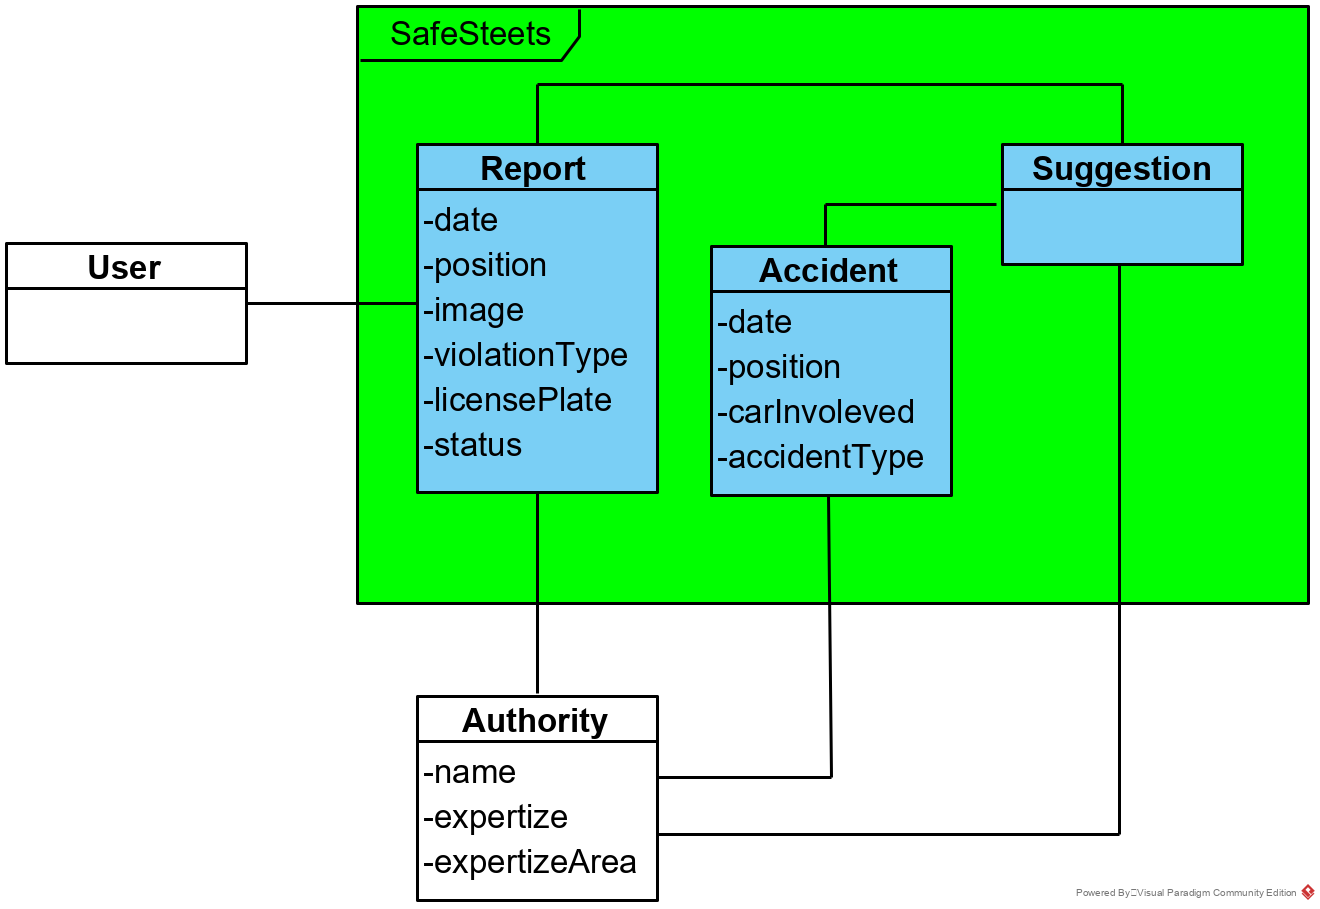
\includegraphics {diagrams/domain_model.png}
				\caption[Domain Model]{Domain Model}
				\label{fig:domain_model}
			\end{figure}
			
			The users can report traffic violations through the SafeStreets application.
			SafeStreets does not collect any data about users, so they are represented as a black box. The interaction between users and SafeStreets is established only through a report, which is published in the SafeStreets system.\\\\
			A registered authority can be noticed about traffic violations reported in its own operative area and eventually evaluate if that traffic violation report is valid or not. Moreover, an authority can report to SafeStreets any information about accidents in order to identify unsafe areas and suggest possible interventions.\\\\
			To understand the main events in SafeStreets system, some statechart diagrams are represented in figures below. \\\\
			\clearpage
			Figure \ref{fig:statechart_userReporting} explains how SafeStreets works when a user try to report a traffic violation.
			
			\begin{figure}[H]
				\centering
				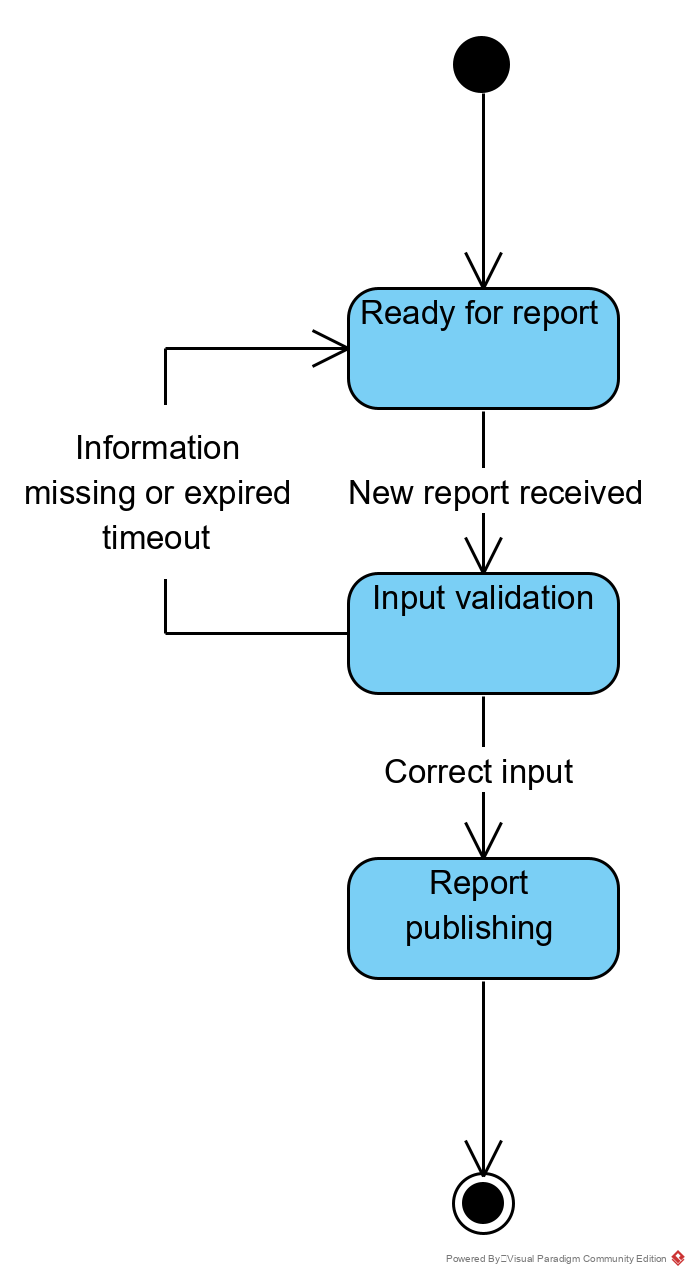
\includegraphics[width=0.5\textwidth]{diagrams/statechart_UserSS.png}
				\caption[Statechart Diagram1]{State chart Diagram about user report.}
				\label{fig:statechart_userReporting}
			\end{figure}
			
			The core of the application is based on user reports: the more reports there are, the more the system can provide information about areas in a municipality. If the app considers a report valid, then it is made public.
			
			\begin{figure}[H]
				\centering
				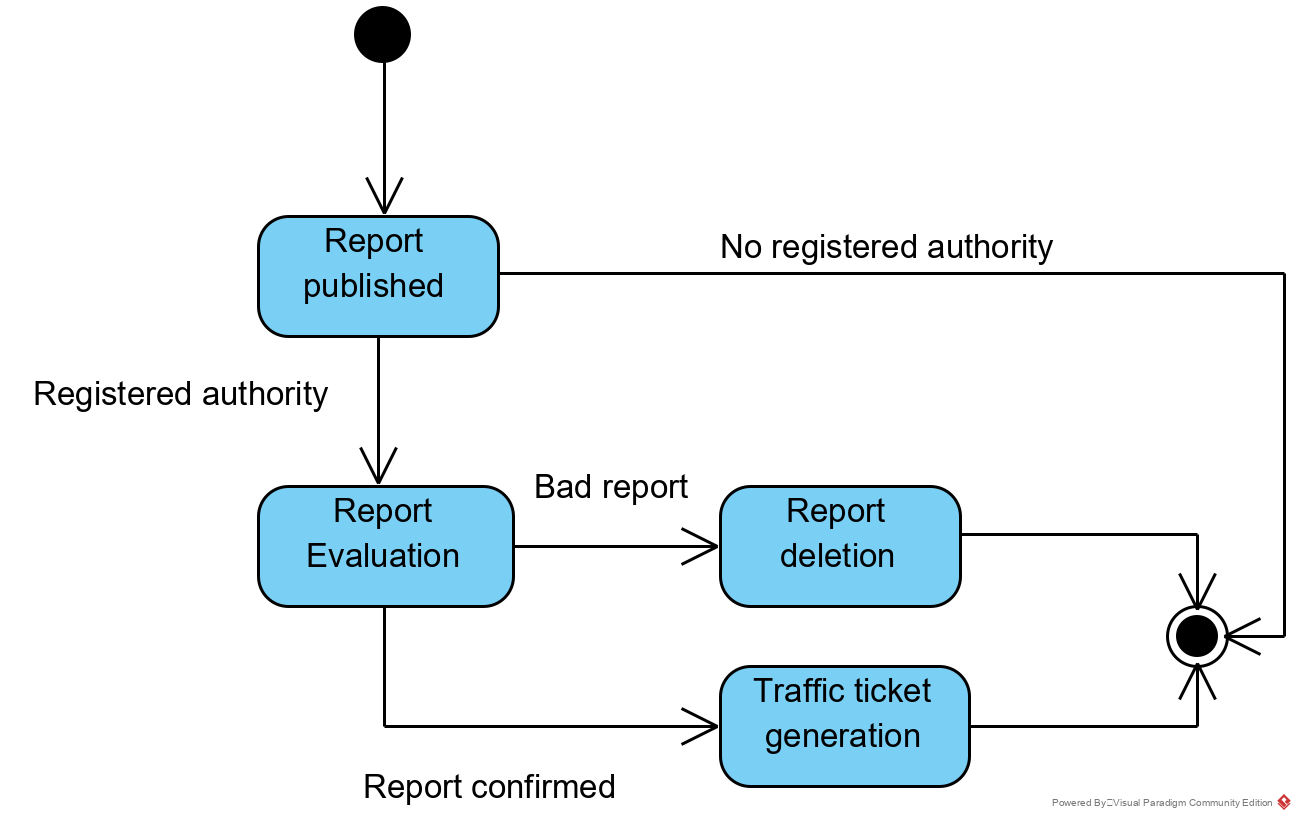
\includegraphics {diagrams/statechart_AuthoritySS.png}
				\caption[State chart Diagram2]{State chart Diagram about SafeStreets suggestions for an authority.}
				\label{fig:statechart_SuggestionsForAuthority}
			\end{figure}
			
			Figure \ref{fig:statechart_SuggestionsForAuthority} shows how SafeStreets operates with an authority.\\
			Authorities could eventually have some information about accidents in their operative zone and can decide to share them with SafeStreets.\\
			SafeStreets collects these data and try to cross them with reports about traffic violations: if for an area there are frequent violations or accidents, SafeStreets suggests possible interventions.
			
			\clearpage
			
			\begin{figure}[H]
				\centering
				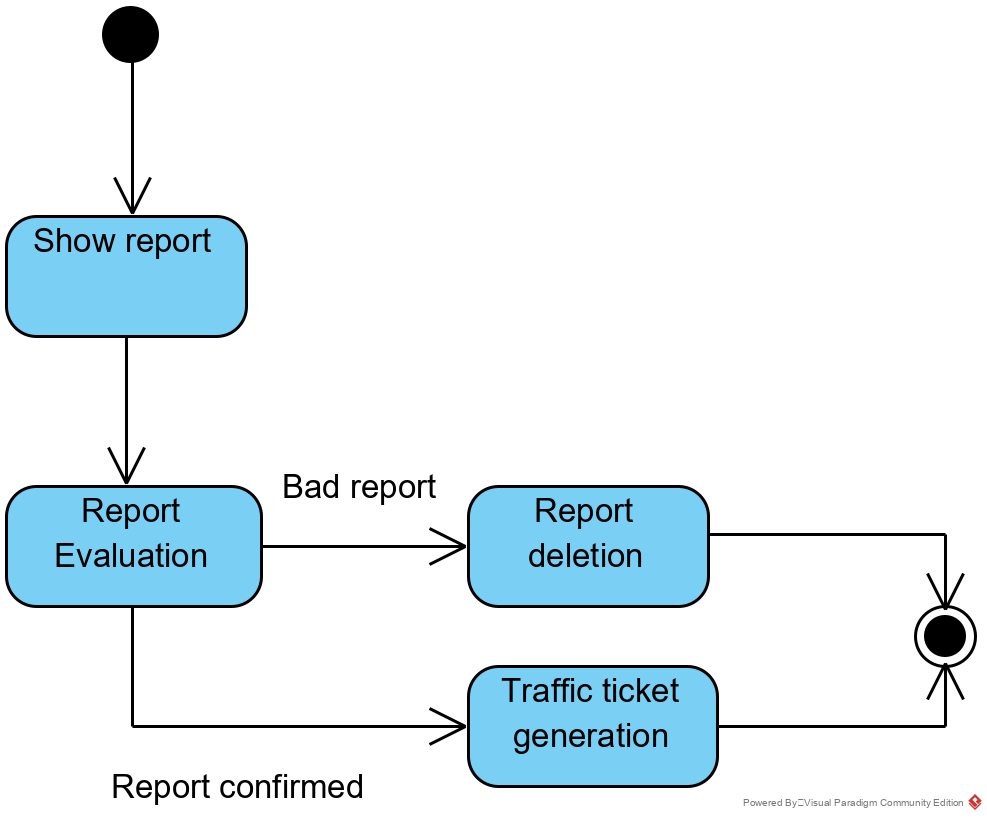
\includegraphics {diagrams/statechart_trafficTicket.png}
				\caption[Statechart Diagram3]{State chart Diagram about SafeStreets system for traffic tickets generation.}
				\label{fig:statechart_trafficTickets}
			\end{figure}
			
			Finally, Figure \ref{fig:statechart_trafficTickets} represents SafeStreets system that allows an authority to show all violations reported in its operative area. Analysing a report, an authority can establish if it is actually valid in order to generate a traffic ticket for the offender. Otherwise, if report is not valid, the authority can delete it.
			
			\clearpage	   
	
		\subsection{Product functions}
			In the following section all the main product functions are defined. The reporting and data-mining functions are considered the main ones, while the other are advanced ones offered by SafeStreets thanks to the collaboration with authorities. Thus, if authorities, in a defined area, are not sharing information with SafeStreets, these advanced functions are not available in that area.
			
			\subsubsection{Violation reporting}
				This is the core function of SafeStreets. The aim is to give to the user the possibility to report a traffic violation. The system allows the user to use this function without any previous login. The user is asked to complete his reporting action defining the following fields:\\
				- Picture representing the violation;\\
				- Type of violation.\\
				Other important information such as position, date and time of the violation are automatically detected by the application.\\
				In particular, to take the requested picture, the user is allowed only to use the in-app dedicated camera tool in order to prevent users from reporting past violations uploading old pictures and to avoid picture manipulations.\\ The picture is approved by the app if and only if the license plate is correctly recognized by the dedicated algorithm, otherwise, the app will ask to the user to take it again.
				\\The type of violation is selectable only by the ones offered by SafeStreets.\\ The user is asked also to complete these two requests in a defined interval of time in order to guarantee the consistency of the report offered to SafeStreets.\\
				When a violation is correctly filled in, it is sent to the system which will publish it and will make it visible to all users.\\
				If an authority that covers the zone in which the violation occured is registered to SafeStreets, then the report is sent to it for evaluation.
		
			\subsubsection{Data-mining}
				This function allows the user to analyse SafeStreets data in order to mine some information, for example, by highlighting the streets (or the areas) with the highest frequency of violations. The kind of information requested can be filtered by user in order to restrict the research area.\\
				Furthermore, SafeStreets can provide to authorities statistics about vehicles, not accessible to common users, for example about the most egregious offenders, or the effectiveness of the SafeStreets initiative by looking for trends in the issuing of tickets.\\
				
			\subsubsection{Accidents collector}
				This function is available only for authorities that manage accidents. They are allowed to enrich SafeStreets' data inserting information about accidents in the competent area. This function will be useful for the interactive suggestion function defined below. 
			
			\subsubsection{Interactive suggestions}
				This function is strictly related to the collaboration between SafeStreets data, offered by users' reports, and authorities, which can enrich the database including information about the accidents that occur. \\SafeStreets can cross all these information and it can also identify potentially unsafe areas suggesting possible interventions to authorities. \\
				In a more detailed way, this function, analyzing data and making a comparison between them and some defined limit parameters, can automatically detect possible standard-defined improvements, create suggestions useful to reduce violations and accidents.
				
			\subsubsection{Report confirmation}
				SafeStreets forwards a report received from a user to an authority that covers the area of the report, if such authority is registered to the system.\\
				Then, the authority can evaluate it: if the report is considered valid, then SafeStreets updates the status of that report as "confirmed", assuming the authority has generated a traffic ticket from it.\\
				If the report is considered not valid, SafeStreets deletes it from the system.\\
				
		\subsection{User characteristics}
			The actors of the application are the following:
			\begin{itemize}
				\item User: a person that is using SafeStreets app. He is a "guest" because he is not logged in, so no specific information about him are given. He can actively use the first two basic functions so he can send a violation reporting or do data-mining.
				\item Authority: special kind of user. It is allowed to use the user functions but it has also additional privileges on them such as to visualize more detailed information about reports. In particular, it is a registered identity that is responsible to manage reports addressed to its area of competence.\\
				An authority can send information about accidents of its area of competence to SafeStreets and can use SafeStreets statistics to identify the most egregious offenders.\\
		        A kind of authority is the police, that can use reports to make traffic tickets validating SafeStreets reports.
			\end{itemize}
		
		\subsection{Assumptions, dependencies and constraints}	\label{assumptions}
			This section specifies the assumptions made in the rest of the document, that is those facts that have been considered true a priori and that are not manageable by SafeStreets.
			\begin{itemize}
				\assumption{1} The device on which the SafeStreets client is installed has internet access.
				\assumption{2} The device on which the app is installed has geolocation features.
				\assumption{3} The device on which the app is installed has an external camera.
				\assumption{4} The device on which the app is installed is able to detect its position with a maximum error of five meters.
				\assumption{5} The position detected by the app coincides with the actual position detected by the geolocalizer.
				\assumption{6} The algorithm used by SafeStreets for reading a license plate from an image reads the correct number plate, if it is present in the image.
				\assumption{7} SafeStreets AE can only be used by the authorities themselves: it is not possible for an unauthorized user to gain access to such software.
				\assumption{8} Each position on earth can be associated with a unique postal code.
				\assumption{9} If an authority confirms a violation report, than the authority generates a traffic ticket from it. So, from the point of view of SafeStreets, every confirmed violation report equals to a traffic ticket.
				\assumption{10} The device on which the SafeStreets Authority Edition is installed is always switched on.
			\end{itemize}
	
	\section{Specific requirements}
		This section contains all the requirements of SafeStreets, i.e. all that allows the app to function as desired by the developer. The requirements depend exclusively on the choices of the developer. Aspects not controllable by the developer, but relevant for the application, are the assumptions reported in \ref{assumptions}.
		
		\subsection{External Interfaces Requirements}
		
			\subsubsection{User Interfaces}
		    The following mockups give an approximate idea of how the interfaces of the application should appear. In the fist block main SafeStreets application interfaces are shown. In the second one main SafeStreets Authority Edition interfaces are shown.
			
			\begin{figure}
				\centering
				\subfloat[][\emph{Welcome page, starting the application}]
				{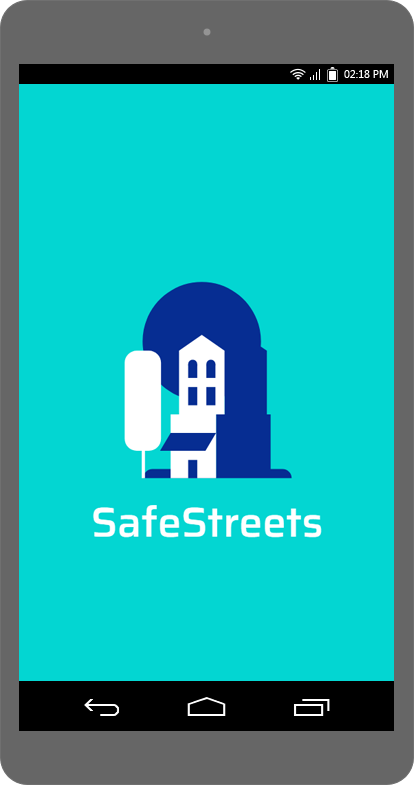
\includegraphics[width=.35\textwidth]{mock/SafeStreetsApplication/1.Welcome.png}} \quad \quad
				\subfloat[][\emph{Application Home Page. The two main function are shown to the user.}]
				{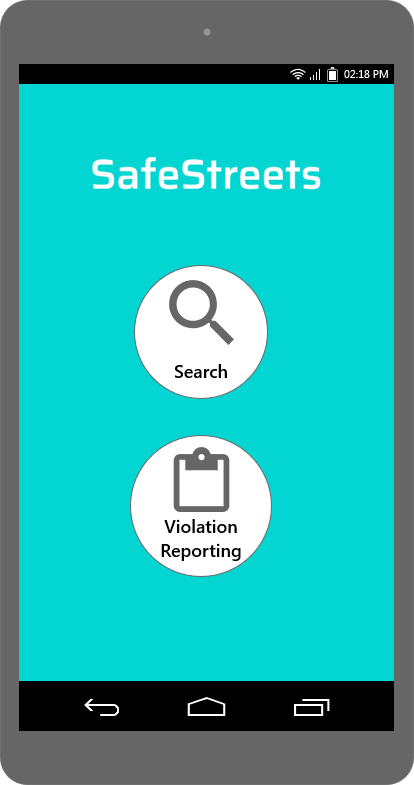
\includegraphics[width=.35\textwidth]{mock/SafeStreetsApplication/2.Home.png}} \\
				\clearpage
				\subfloat[][\emph{Violation Reporting: Take Picture}]
				{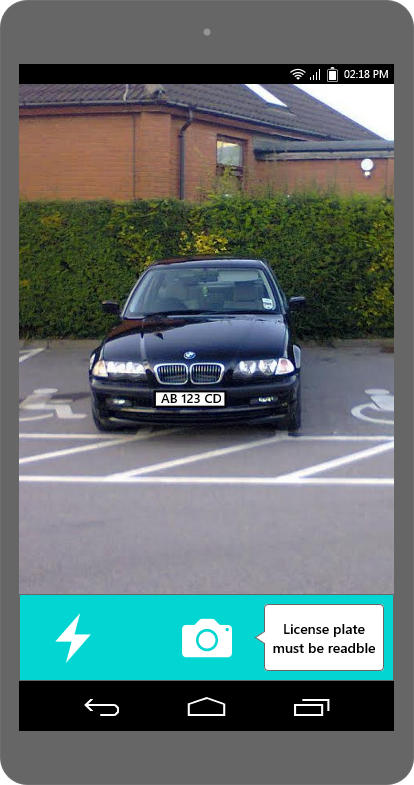
\includegraphics[width=.35\textwidth]{mock/SafeStreetsApplication/4.TakePhoto.png}} \quad \quad
				\subfloat[][\emph{Violation Reporting: Metadata acquired from picture + Violation Type selection}]
				{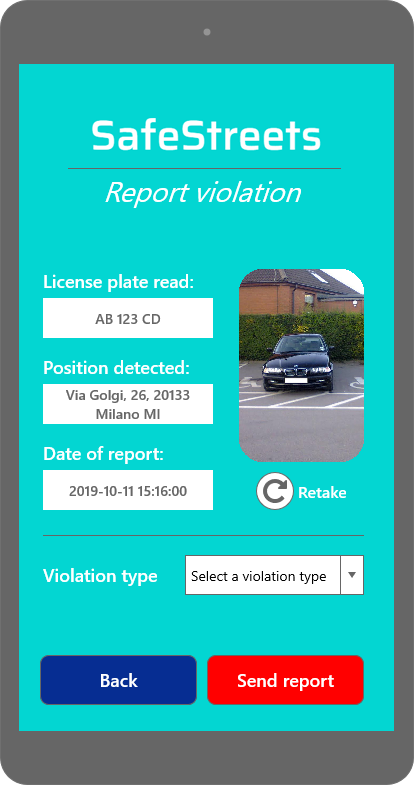
\includegraphics[width=.35\textwidth]{mock/SafeStreetsApplication/5.ReportViolation.png}} \\
	
				\caption{SafeStreets application interfaces}
				\label{fig:app_interfaces}
			\end{figure}

			
			\begin{figure}
				\centering
				\subfloat[][\emph{Data Mining: browse map}]
				{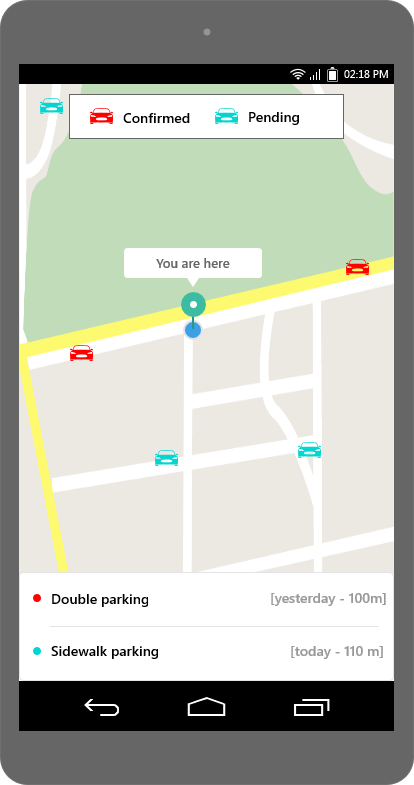
\includegraphics[width=.35\textwidth]{mock/SafeStreetsApplication/3.Search.png}} \quad \quad
				\subfloat[][\emph{Data Mining: side menu filters}]
				{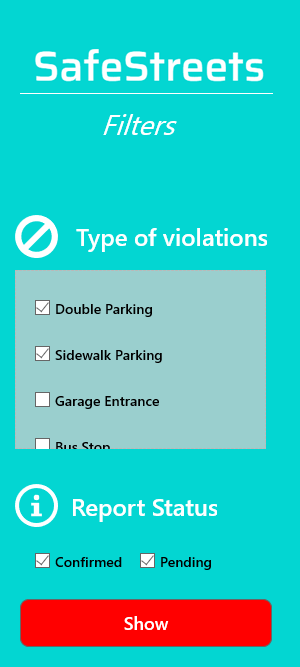
\includegraphics[width=.35\textwidth]{mock/SafeStreetsApplication/3b.sideMenuFilters.png}} \\			
				\caption{SafeStreets application interfaces}
				\label{fig:app_interfaces2}
			\end{figure}

		
			\begin{figure}
				\centering
				\subfloat[][\emph{Welcome page, starting the AE system}]
				{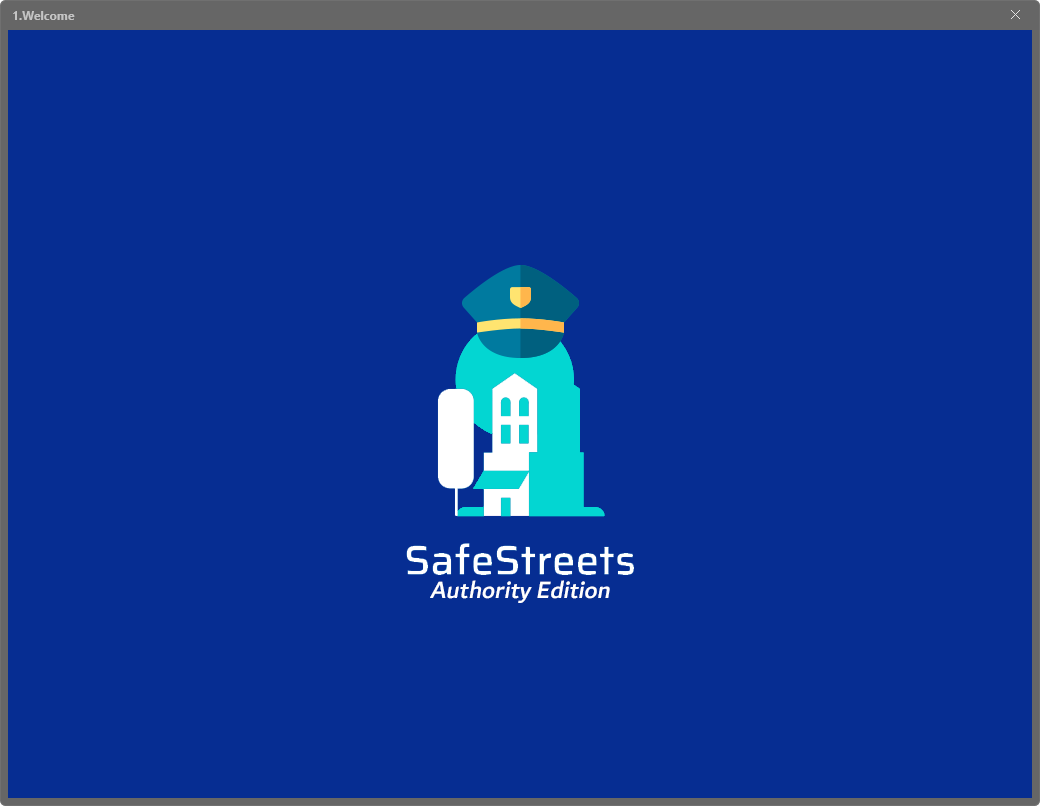
\includegraphics[width=.90\textwidth]{mock/SafeStreetsAE/1.Welcome.png}} \quad \quad
				\subfloat[][\emph{Home Page}]
				{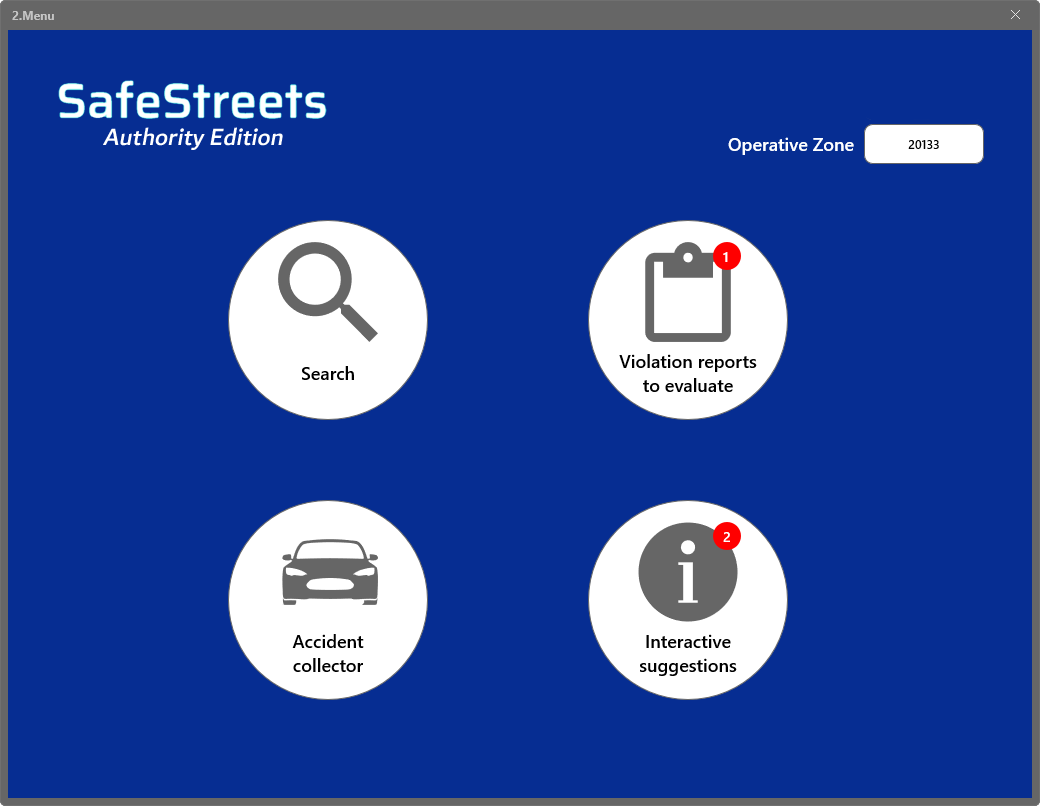
\includegraphics[width=.90\textwidth]{mock/SafeStreetsAE/2.Menu.png}} \\			
				\caption{SafeStreets Authority Edition interfaces}
				\label{fig:AE_interfaces}
			\end{figure}

			\begin{figure}
				\centering
				\subfloat[][\emph{Report Evaluation}]
				{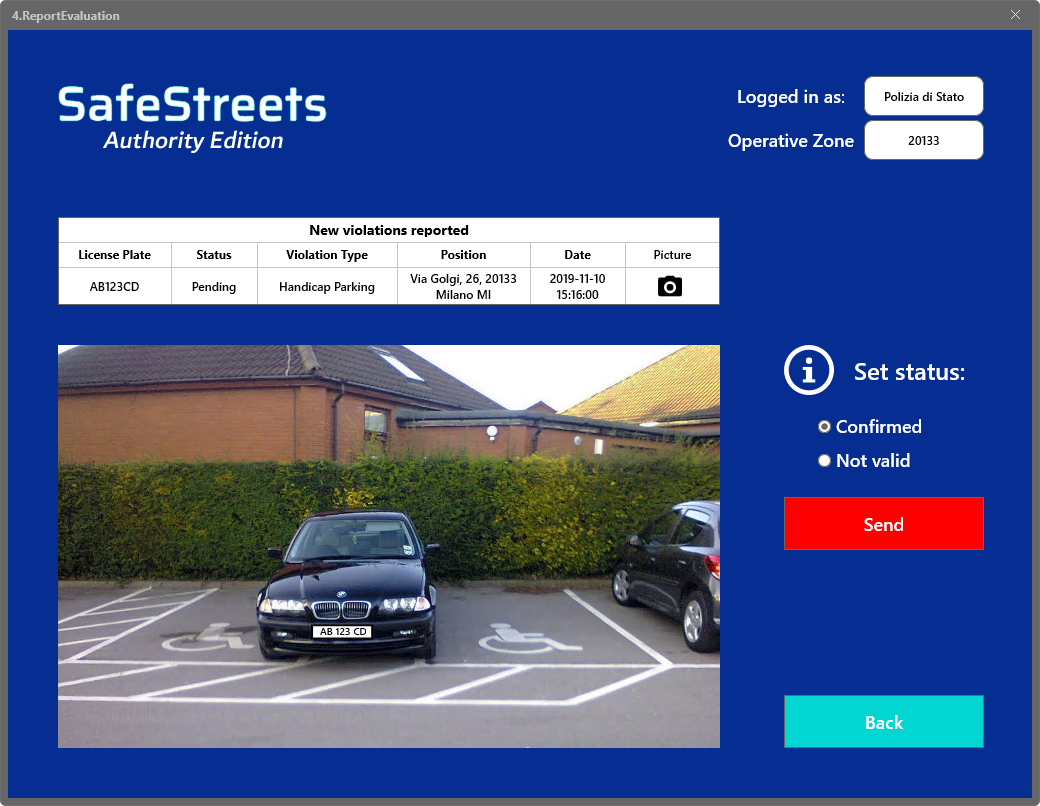
\includegraphics[width=.90\textwidth]{mock/SafeStreetsAE/4.ReportEvaluation.png}} \quad \quad
				\subfloat[][\emph{Data Mining}]
				{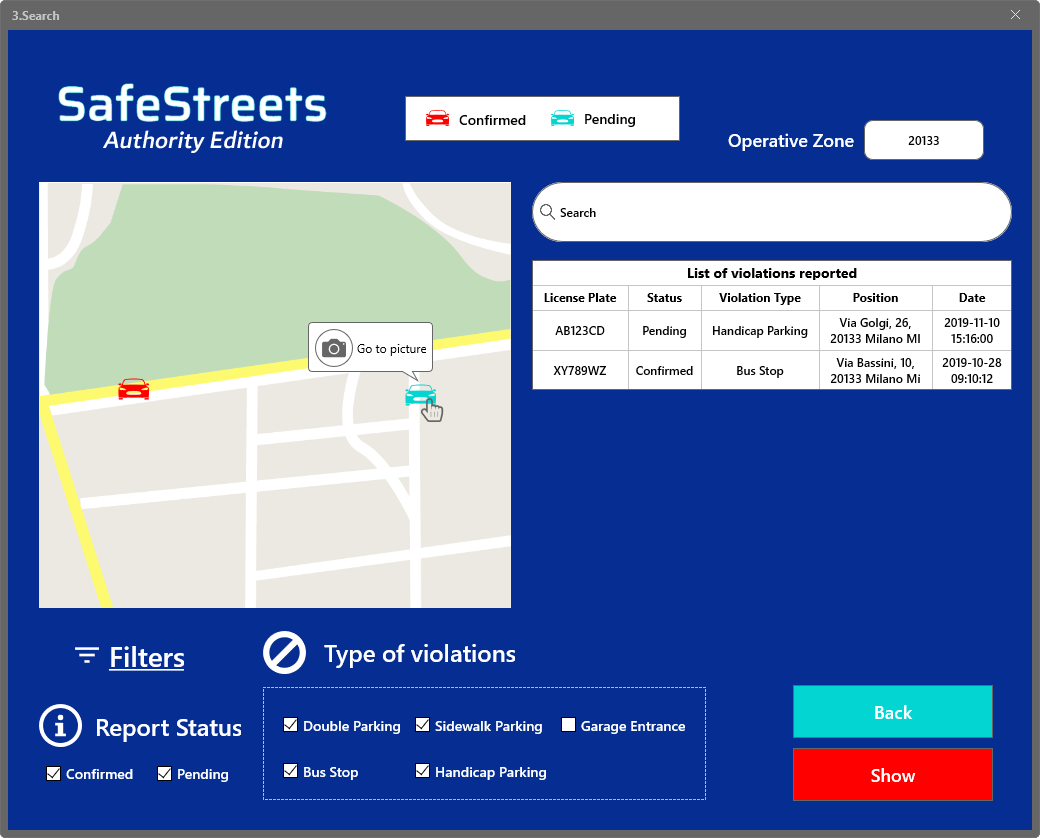
\includegraphics[width=.90\textwidth]{mock/SafeStreetsAE/3.Search.png}} \\			
				\caption{SafeStreets Authority Edition interfaces}
				\label{fig:AE_interfaces2}
			\end{figure}

		
			\begin{figure}
			\centering
			\subfloat[][\emph{Accident Collector}]
			{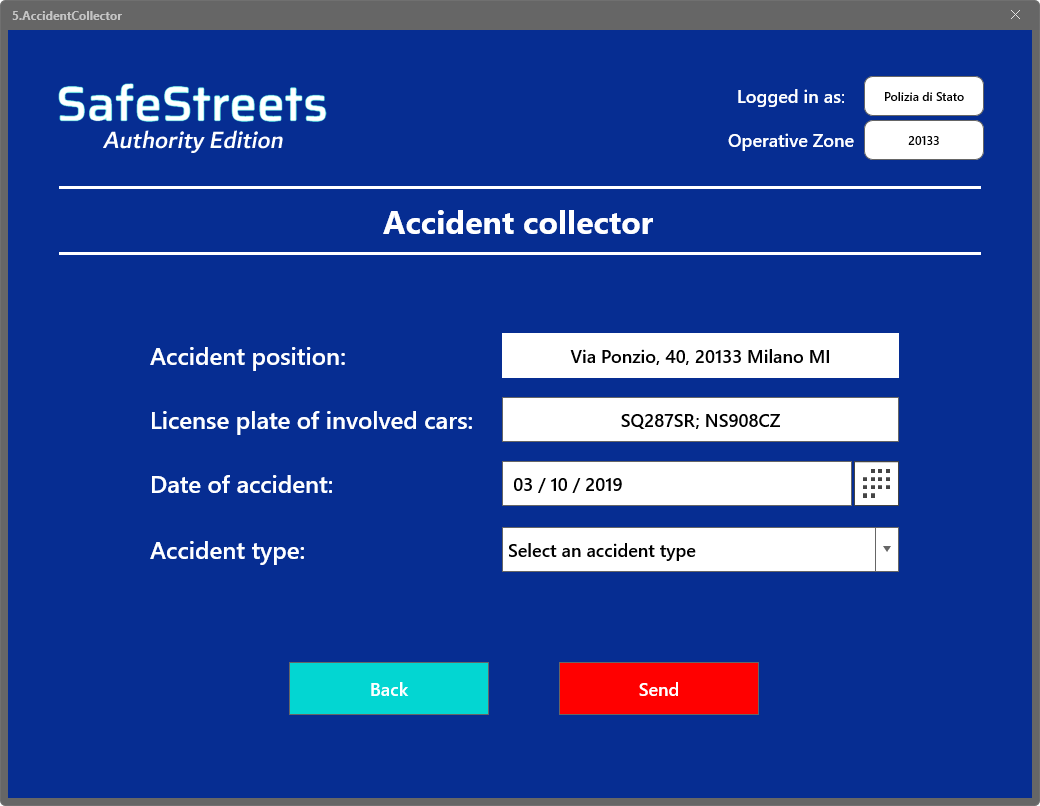
\includegraphics[width=.90\textwidth]{mock/SafeStreetsAE/5.AccidentCollector.png}} \quad \quad
			\subfloat[][\emph{Interactive Suggestions}]
			{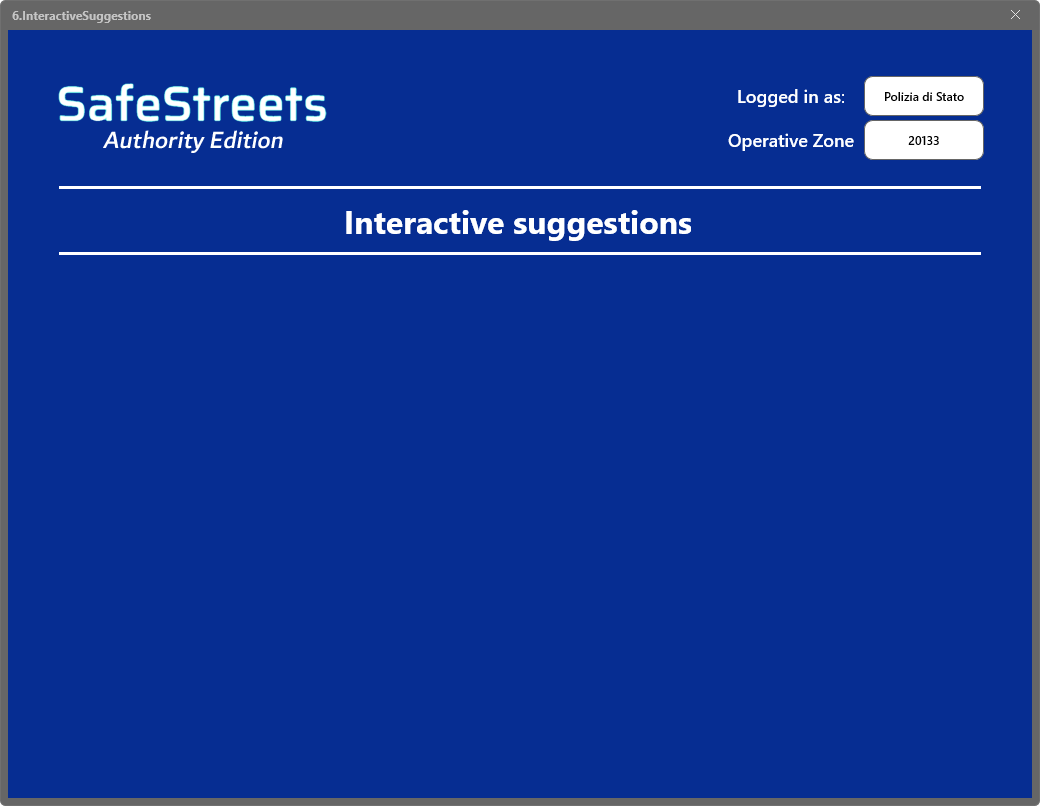
\includegraphics[width=.90\textwidth]{mock/SafeStreetsAE/6.InteractiveSuggestions.png}} \\			
			\caption{SafeStreets Authority Edition interfaces}
			\label{fig:AE_interfaces2}
		\end{figure}

			
			
			\subsubsection{Hardware Interfaces} \label{hardware_interfaces}
				Since SafeStreets is a crowd-sourced application, each user could take advantage of the system only if it has a smartphone. In particular, the smartphone must have an external camera, GPS and an internet connection.
				Without the camera or the GPS, it is not possible to report violations. Without an internet connection, every SafeStreets function isn't available.
				
			\subsubsection{Software Interfaces}
				First of all, SafeStreets must be authorized by the operating system of the smartphone on which it is installed to access the camera, the GPS and the internet connection.\\
				\\
				In order to provide information about traffic violations to users, SafeStreets uses external maps to show where reports come from. SafeStreets gets these maps from OpenStreetMap (\url{https://www.openstreetmap.org}).\\
				\\
				Moreover, one of the element to ensure that a report could be formalized is the validation of license plate. SafeStreets takes advantage of an algorithm to automatically recognize characters on license plates (OCR Algorithm).
				
				
			\subsubsection{Communication Interfaces}
				Each function provided by SafeStreets needs an Internet connection.
		\subsection{Functional Requirements}
			In the current section will be shown for each goal the list of functional requirements and the assumptions to be respected.
			
			\begin{itemize}
				\goal{1}An individual can report traffic violations to SafeStreets.
				\begin{itemize}
					\assumption{1} The device on which the SafeStreets client is installed has internet access.
					\assumption{2} The device on which the app is installed has geolocation features.
					\assumption{3} The device on which the app is installed has an external camera.
					\assumption{4} The device on which the app is installed is able to detect its position with a maximum error of five meters.
					\assumption{5} The position detected by the app coincides with the actual position detected by the geolocalizer.
					\assumption{6} The algorithm used by SafeStreets for reading a license plate from an image reads the correct number plate, if it is present in the image.
					\assumption{7} Each position on earth can be associated with a unique postal code.
					\assumption{8} The SafeStreets client must be able to communicate with the SafeStreets system.
					\assumption{9} The only license plate shown in the report image is the one of the offender.
					\assumption{10} Each violation report must refer to only one offender.	
					\requirement{1} The user report must be of one of the type of violation defined by SafeStreets.
					\requirement{2} The report image must show the license plate of the offender.
					\requirement{3} The user must insert the picture of the violation.
					\requirement{4} The user must complete the report before the expiration of the report timeout.
					\requirement{5} The OCR algorithm must detect one license plate into the report image.
					\requirement{6} The APP must detect automatically position and date. 
					\requirement{7} Every violation report sent to server must be filled in all its fields.
					\requirement{17} Every violation reported to SafeStreets is consistently saved into the SafeStreets database.
					
				\end{itemize}
				\goal{2}An individual can mine information about violations.
				\begin{itemize}
					\assumption{1} The device on which the SafeStreets client is installed has internet access.
					\assumption{11} If an authority confirms a violation report, than the authority generates a traffic ticket from it. So, from the point of view of SafeStreets, every confirmed violation report equals to a traffic ticket.
					\requirement{8} The SafeStreets client must show all and only the information required by the individual.
					\requirement{9} Every individual can browse the map.
					\requirement{10} Every individual can see statistics in map.
					\requirement{11} Every individual can define filters for the research.
					\requirement{12} Every authority can see advanced statistics in map (including sensitive information).
					\requirement{13} Every authority can define advanced filters for the research (including sensitive information).
					
				\end{itemize}					
				\goal{3}An authority can share its information about accidents occurred on its operative area with SafeStreets.
				\begin{itemize}
					\assumption{1} The device on which the SafeStreets client is installed has internet access.
					\assumption{7} Each position on earth can be associated with a unique postal code.
					\assumption{12} The SafeStreets software installed in the offices of the authorities registered with the service can only be used by the authorities themselves: it is not possible for an unauthorized user to gain access to such software.
					\assumption{13} The device on which the SafeStreets Authority Edition is installed is always switched on.
				   \requirement{14} The information about accidents must be of one of the type defined by SafeStreets.
				   \requirement{15} Information about accidents occurred must include all the information required by SafeStreets.
				   \requirement{16} Every accident reported by a registered authority is consistently saved into the SafeStreets database.
				\end{itemize}
				\goal{4}An authority can retrieve suggestions of possible interventions from SafeStreets.
				\begin{itemize}
					\assumption{1} The device on which SafeStreets client is installed has internet access.
					\assumption{12} SafeStreets software installed in the offices of the authorities registered with the service can only be used by the authorities themselves: it is not possible for an unauthorized user to gain access to such software.
					\assumption{13} The device on which SafeStreets Authority Edition is installed is always switched on.
					\requirement{18} SafeStreets must be able to generate suggestions, based on accidents and confirmed violation reports.
					\requirement{19} Every authority must receive suggestions only referred to its operative area.
				\end{itemize}
				\goal{5}An authority can evaluate SafeStreets reports related to its area of competence.
				\begin{itemize}
					\assumption{1} The device on which the SafeStreets client is installed has internet access.
					\assumption{11} If an authority confirms a violation report, than the authority generates a traffic ticket from it. So, from the point of view of SafeStreets, every confirmed violation report equals to a traffic ticket.
					\assumption{12} SafeStreets software installed in the offices of the authorities registered with the service can only be used by the authorities themselves: it is not possible for an unauthorized user to gain access to such software.
					\assumption{13} The device on which the SafeStreets Authority Edition is installed is always switched on.
					\requirement{20} An authority receives a report if and only if that report is related to a position covered by that authority (i.e. the postal code of the position of the violation report is assigned to that authority).
					\requirement{21} When a registered authority confirms a violation report, that confirmation is consistently stored into the server.
					\requirement{22} A violation report rejected by a registered authority is removed from SafeStreets database.
				\end{itemize}
			\end{itemize}
		
			\subsubsection{Use Case Diagrams}
				In this section the use case of the system is shown.
				\begin{figure}[H]
					\centering
					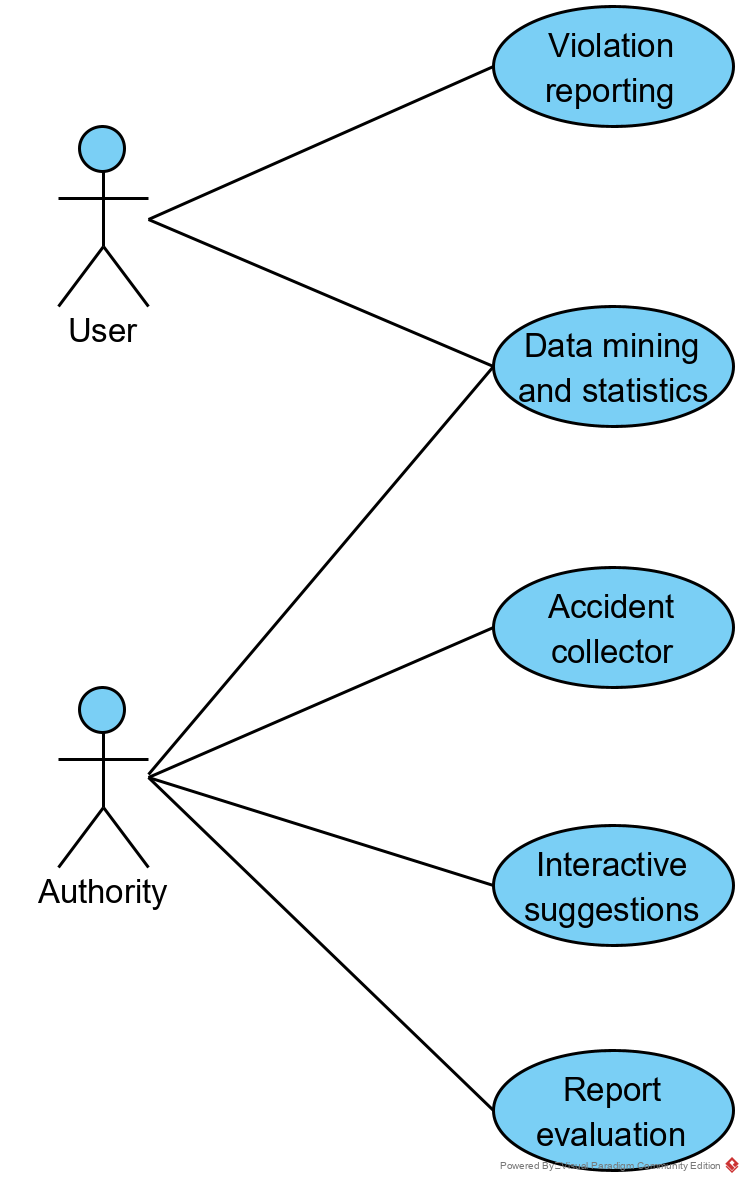
\includegraphics[width=0.8\textwidth]{diagrams/usecase_safestreets.png}
					\caption[SafeStreets use case diagram]{SafeStreets Use Case Diagram}
					\label{fig:usecase_safestreets}
				\end{figure}
			
			\clearpage
			\subsubsection{Use Case Description}
				
				\textbf{ID}: \usecase{1} \\
				\textbf{Name}:   Violation reporting\\
				\textbf{Actor}:  User\\
				\textbf{Entry conditions}:
				\begin{enumerate}
					\item Open the SafeStreets application.
					\item Open the "Violation reporting" section.
				\end{enumerate}
				\textbf{Event flow}:
				\begin{enumerate}
					\item The app opens the camera to take the picture of the violation. Take the picture. When the picture is taken, the reporting timeout starts.
					\item The app shows the taken picture and the license plate read from it by the license plate recognition algorithm. If the user is not satisfied by the result, he can take a new picture clicking on the button "take picture". The reporting timeout is restarted every time a picture is taken.
					\item Choose a "type of violation" from the list of violations recognized by SafeStreets. The user cannot define itself a type of violation.
				\end{enumerate}
				\textbf{Exit conditions}:
				\begin{itemize}
					\item The user can always leave the violation reporting function clicking on the "Back" button. In this way, he returns to the main page of the app.
					\item Click "Send" to complete the violation reporting. The app returns to the main page.
				\end{itemize}
				\textbf{Exceptions}:
				\begin{itemize}
					\item If the camera or the geolocalization service aren't available, the app shows an error message and returns to the main page: it is not possible to send a violation report.
					\item If the license plate recognition algorithm fails, the user is forced to take the picture again.
					\item If the user clicks on "Send" without having filled all the requested fields, the app shows a warning message that tells the user what is wrong. The user can close the warning message and come back to the violation report. 
					\item If the reporting timeout expires before the user has correctly sent the violation report, an error message is shown, than the app discard the violation report and returns to the main page.\\
				\end{itemize}
			
				\rule{\linewidth}{0.4pt}
				\\
				
				\textbf{ID}: \usecase{2} \\
				\textbf{Name}:   Data mining and statistics\\
				\textbf{Actor}:  User, Authority\\
				\textbf{Entry conditions}:
				\begin{enumerate}
					\item User opens the SafeStreets application; authority opens SafeStreets AE.
					\item Open the "Search" section.
				\end{enumerate}
				\textbf{Event flow}:
				\begin{enumerate}
					\item The app shows in a new screen the map. Then, report violations are represented in the map with different coloured pins, based on confirmed or unconfirmed reports. This screen also provides a menu through which either a user or an authority can refine its research with data filters.
					They select the filters they want.
					\item Taps on "Show" button.
					\item Explores data about result reports. In particular:
					\begin{itemize}
						\item A user can retrieve information about type of violation, date, position and eventually the label "confirmed" or "pending".
						\item An authority can retrieve the same information as before, adding license plates and proof pictures.
					\end{itemize}
				\end{enumerate}
				\textbf{Exit conditions}:
				\begin{itemize}
					\item Either user or authority can always leave the "Search" function clicking on the "Back" button. In this way, they return to the main page of the app.
				\end{itemize}
				\textbf{Exceptions}: -\\
				
				\rule{\linewidth}{0.4pt}
				\\
					
				\textbf{ID}: \usecase{3} \\
				\textbf{Name}:   Accident collector\\
				\textbf{Actor}:  Authority\\
				\textbf{Entry conditions}:
				\begin{enumerate}
					\item Open SafeStreets AE.
					\item Open the "Accident Collector" section.
				\end{enumerate}
				\textbf{Event flow}:
				\begin{enumerate}
					\item Compile requested fields: type of accident, offenders' license plate (separated by a semicolon), address of the accident, date of the accident.
				\end{enumerate}
				\textbf{Exit conditions}:
				\begin{itemize}
					\item The authority can always leave the accident collector function clicking on the "Back" button. In this way, it returns to the main page of the app.
					\item Click "Send" to complete the accident compilation form. SafeStreets AE returns to the main page.
				\end{itemize}
				\textbf{Exceptions}:
				\begin{itemize}
					\item Some of the requested form are not correctly compiled or empty. In this case a warning message is shown. The authority can close the warning message and come back to the accident collector.\\
				\end{itemize}
				
				\rule{\linewidth}{0.4pt}
				\\
								
				\textbf{ID}: \usecase{4} \\
				\textbf{Name}:   Interactive suggestions\\
				\textbf{Actor}:  Authority\\
				\textbf{Entry conditions}:
				\begin{enumerate}
					\item Open SafeStreets AE.
					\item Open the "Interactive suggestions" section.
				\end{enumerate}
				\textbf{Event flow}:
				\begin{enumerate}
					\item A list of suggestion are shown.
					\item The authority can mark the read suggestion clicking on the "Got it" button in order to hide the already read suggestions.
				\end{enumerate}
				\textbf{Exit conditions}:
				\begin{itemize}
				   \item The authority can always leave the accident collector function clicking on the "Back" button. In this way, it returns to the main page of SafeStreets AE.
				\end{itemize}
				\textbf{Exceptions}: -\\
				
				\rule{\linewidth}{0.4pt}
				\\
				
				\textbf{ID}: \usecase{5} \\
				\textbf{Name}: Report evaluation\\
				\textbf{Actor}: Authority\\
				\textbf{Entry conditions}:
				\begin{enumerate}
					\item Open SafeStreets AE.
					\item Click on "Violation reports to evaluate".
				\end{enumerate}
				\textbf{Event flow}:
				\begin{enumerate}
					\item If there is at least one report to evaluate, the app shows all the information about the report. Choose between the buttons "Confirmed" and "Not valid". Their meaning is straightforward.
				\end{enumerate}
				\textbf{Exit conditions}:
				\begin{itemize}
					\item Click on the chosen button. If there is another violation report to evaluate, the event flow restarts. Otherwise, SafeStreets AE returns to the main page. Remember that SafeStreets considers every confirmed violation report as a given traffic ticket.
					\item The authority can always leave the violation report confirmation function clicking on the "Back" button. In this way, it returns to the main page of SafeStreets AE.
				\end{itemize}
				\textbf{Exceptions}: -\\
				
			\clearpage
			\subsubsection{Activity diagrams}
			The core of SafeStreets application is based on violation reports by users. \figurename{ \ref{fig:activitydiagram_report}} explains in little steps how a user can do this operation.
			\begin{figure}[H]
				\centering
				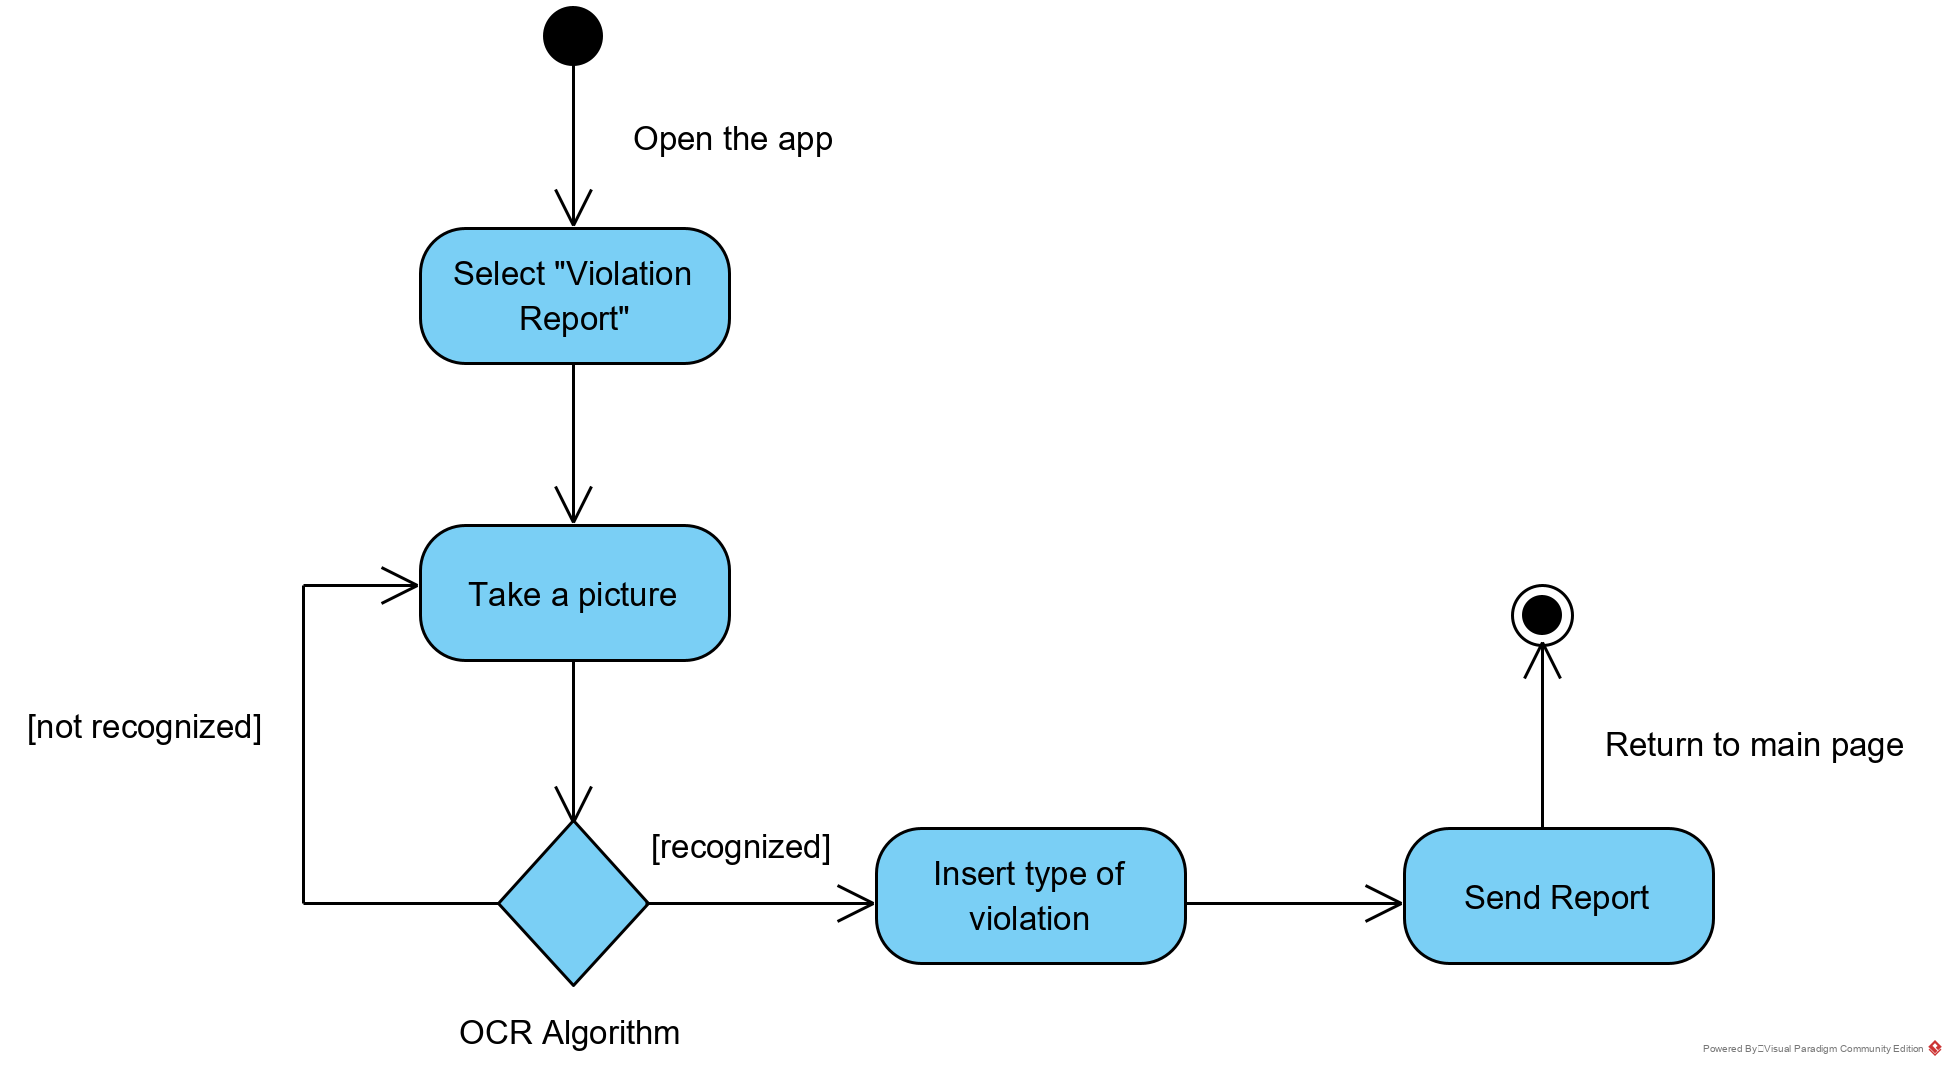
\includegraphics[width=1\textwidth]{diagrams/activity_report.png}
				\caption[SafeStreets activity diagram]{SafeStreets activity diagram for violation reporting}
				\label{fig:activitydiagram_report}
			\end{figure} 
			Opening the SafeStreets application and selecting the "Violation Report" button, the user has to take a photo of the vehicle he thinks it is in a violation condition. The photo must clearly include the license plate of the vehicle.
			An OCR algorithm get the picture and shows the read characters: if the user confirms that the license plate is correct, then proceeds in reporting, otherwise he can take a picture again until he's satisfied.\\
			Proceeding in reporting, the user has given the possibility to choose one of the violation types provided by SafeStreets app. After that, report is sent.\\
			
			\clearpage
			Data mining function (\figurename{ \ref{fig:activitydiagram_datamining}}) is executable either by users or by authorities: the main difference is the visibility level of some information.
			\begin{figure}[H]
				\centering
				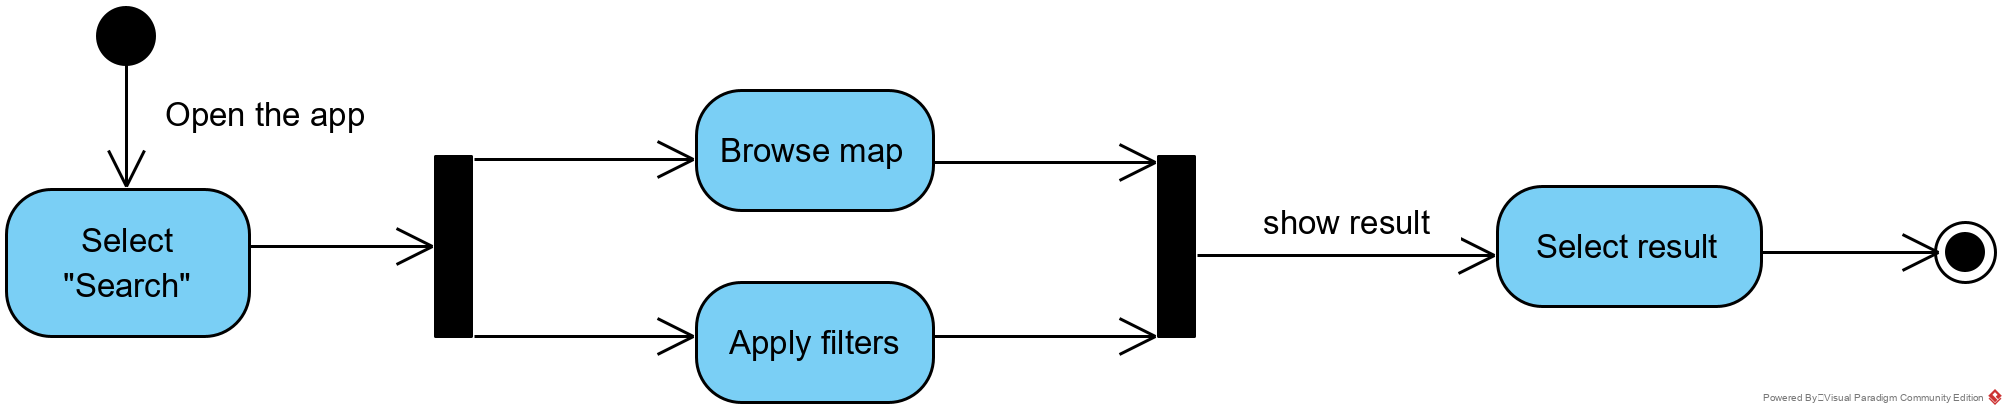
\includegraphics[width=1\textwidth]{diagrams/activity_dataMining.png}
				\caption[SafeStreets activity diagram]{SafeStreets activity diagram for data mining}
				\label{fig:activitydiagram_datamining}
			\end{figure}
			Opening the app (SafeStreets application for users, SafeStreets AE for authority), it is possible to browse information about violation reports, selecting the "Search" button.\\
			Both users and authorities can explore a map of violations position and click to retrieve information about them; moreover, they can specify some additional filter to refine a research.\\
			Finally, results are shown.
			
			\clearpage
			\subsubsection{Sequence Diagrams}
			Let's look at details in interactions between a user and SafeStreets, during the violation reporting phase (\figurename{ \ref{fig:sequencediagram_reporting}}).
			
			\begin{figure}[H]
				\centering
				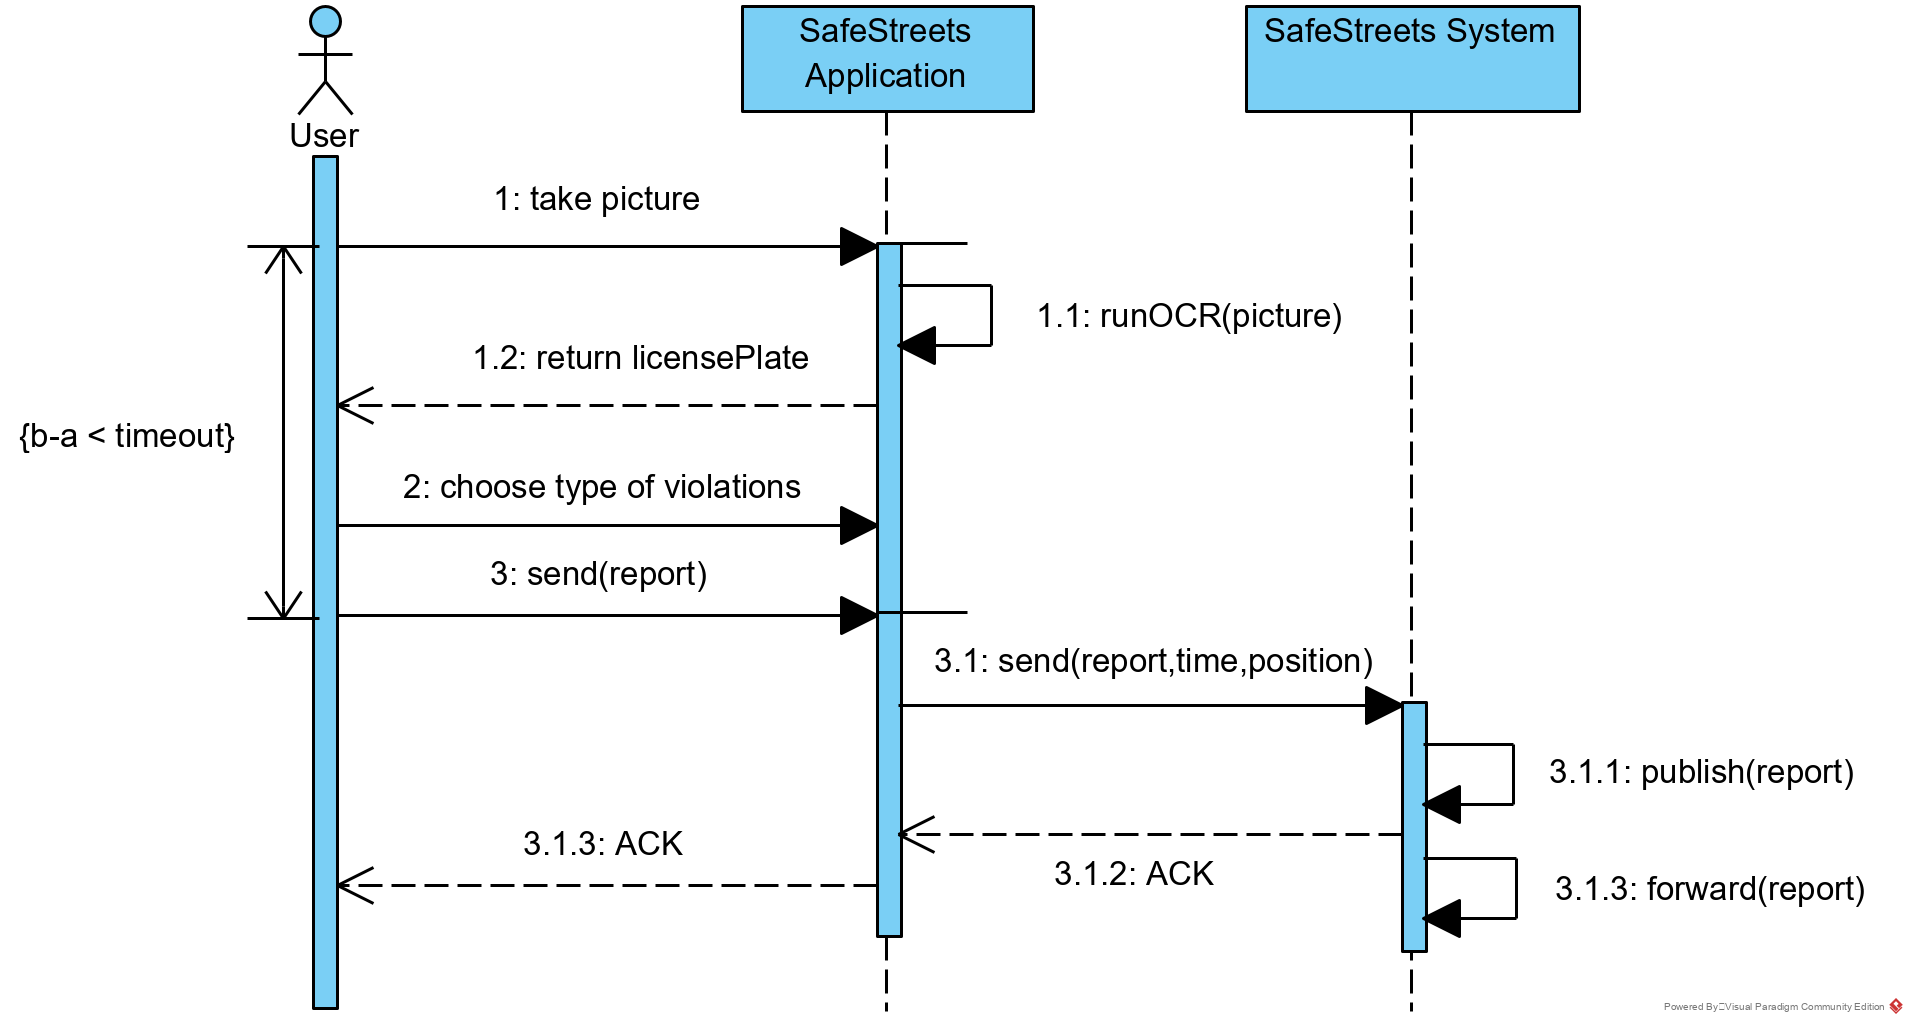
\includegraphics[width=1\textwidth]{diagrams/sequence_reportViolation.png}
				\caption[SafeStreets sequence diagram]{SafeStreets sequence diagram for violation reporting}
				\label{fig:sequencediagram_reporting}
			\end{figure}
			
			Steps from (1) to (3) have been explained in \figurename{ \ref{fig:activitydiagram_report}}: here, an additional information is given representing the time constraint \textit{"b-a"}.\\
			This interval guarantees that a report could be sent about at the same time in which user sees a vehicle in a possible violation condition.\\
			In this way, users can not keep for a long time a report before they send it, so a timeout must be considered.\\
			From step (3.1), the application actually retrieves information about time and position and send the report to SafeStreets system. Then, report will be published and forwarded to the registered authority which operates in the specified position.\\
			 
			 The next two sequence diagrams explain detailed steps about authorities' function, provided by SafeStreets AE.\\\\
			 \figurename{ \ref{fig:sequencediagram_evaluation}} represents that service for authorities, able to manage and evaluate reports sent by users.\\
			 The authority checks if there are new report to evaluate, so, through the application AE, contact SafeStreets system to retrieve these information.\\
			 If there's at least one report to evaluate, SafeStreets AE will show it and permit authorities to establish if the report is correct or not.\\
			 If it is correct, the system will update the report status, checking it as "Confirmed"; otherwise SafeStreets system will remove that report.\\
			
			\begin{figure}[H]
				\centering
				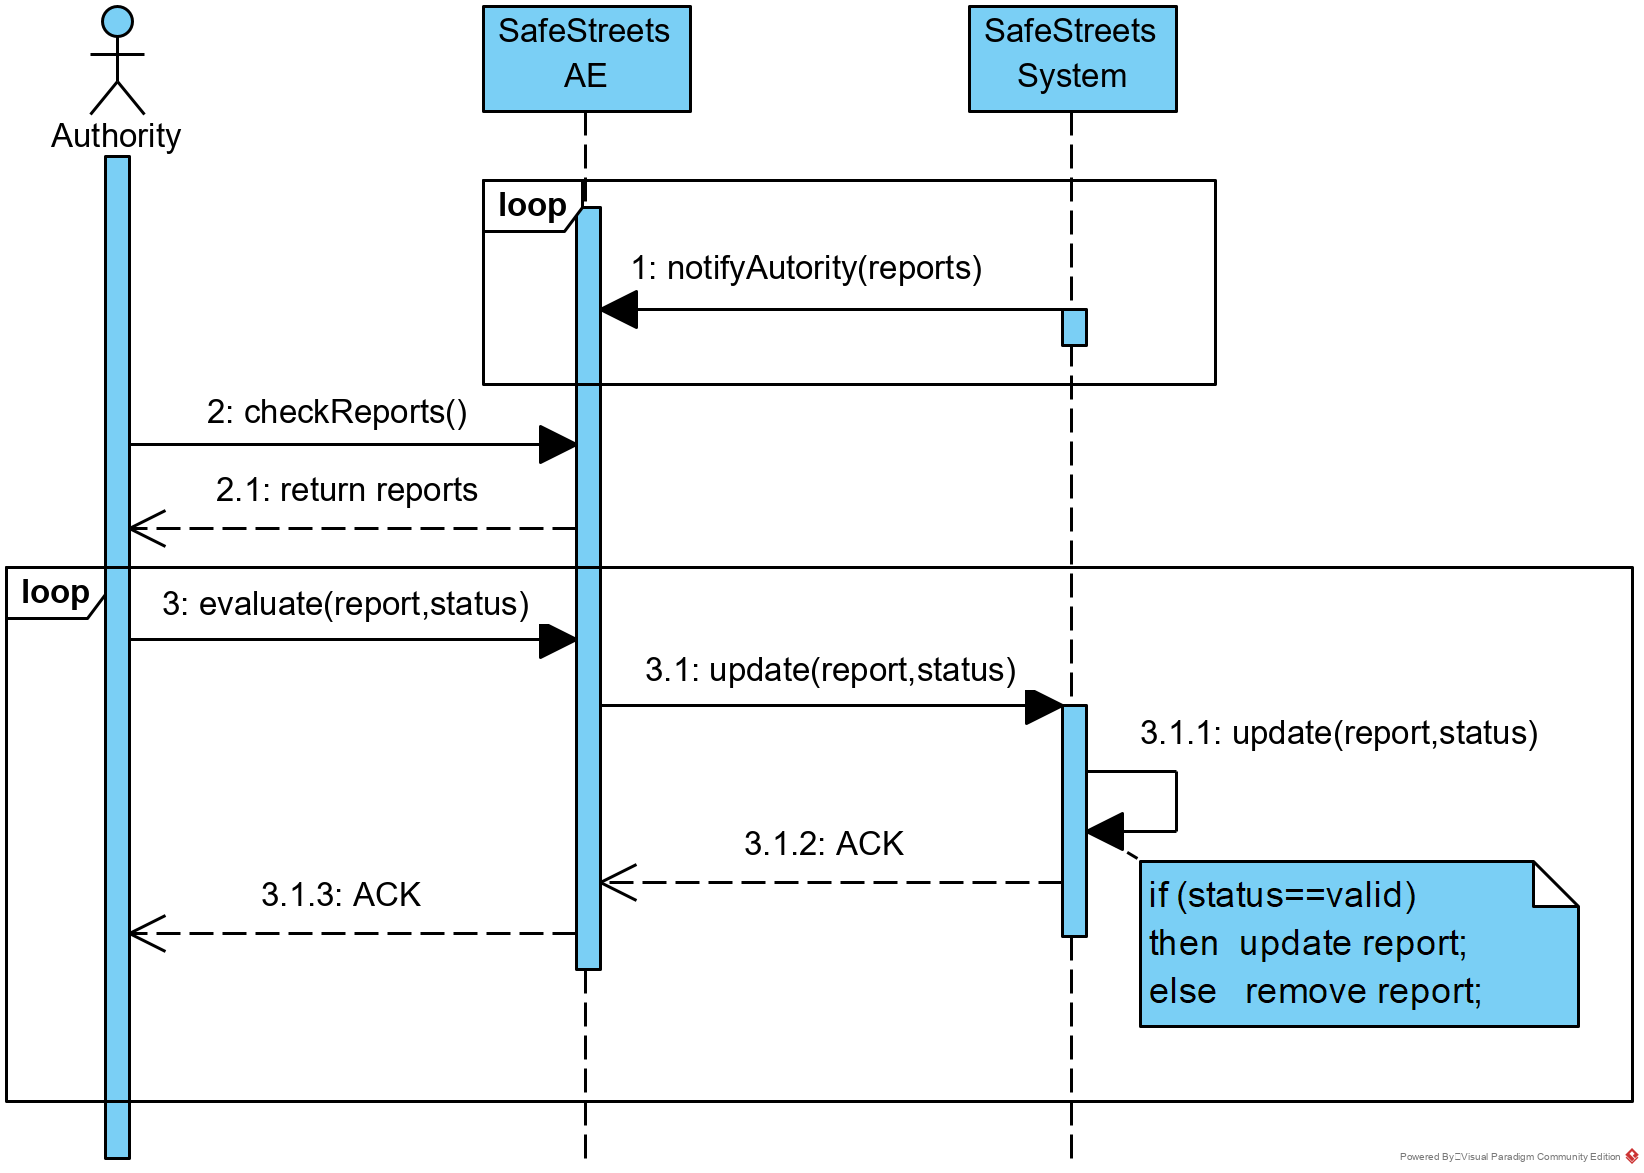
\includegraphics[width=1\textwidth]{diagrams/sequence_evaluateReport.png}
				\caption[SafeStreets sequence diagram]{SafeStreets sequence diagram for report evaluation}
				\label{fig:sequencediagram_evaluation}
			\end{figure}
		
			Finally, an authority can eventually insert in SafeStreets system information about accidents occurred in its operative area.\\
			Gradually, SafeStreets system collect these data and cross them with report violations: once it has analyzed enough data, SafeStreets system will generate for the authority a set of suggestions, aimed to secure the area. \\\\
			\figurename{ \ref{fig:sequencediagram_suggestions}} describes the just mentioned functionality.
			
			\begin{figure}[H]
				\centering
				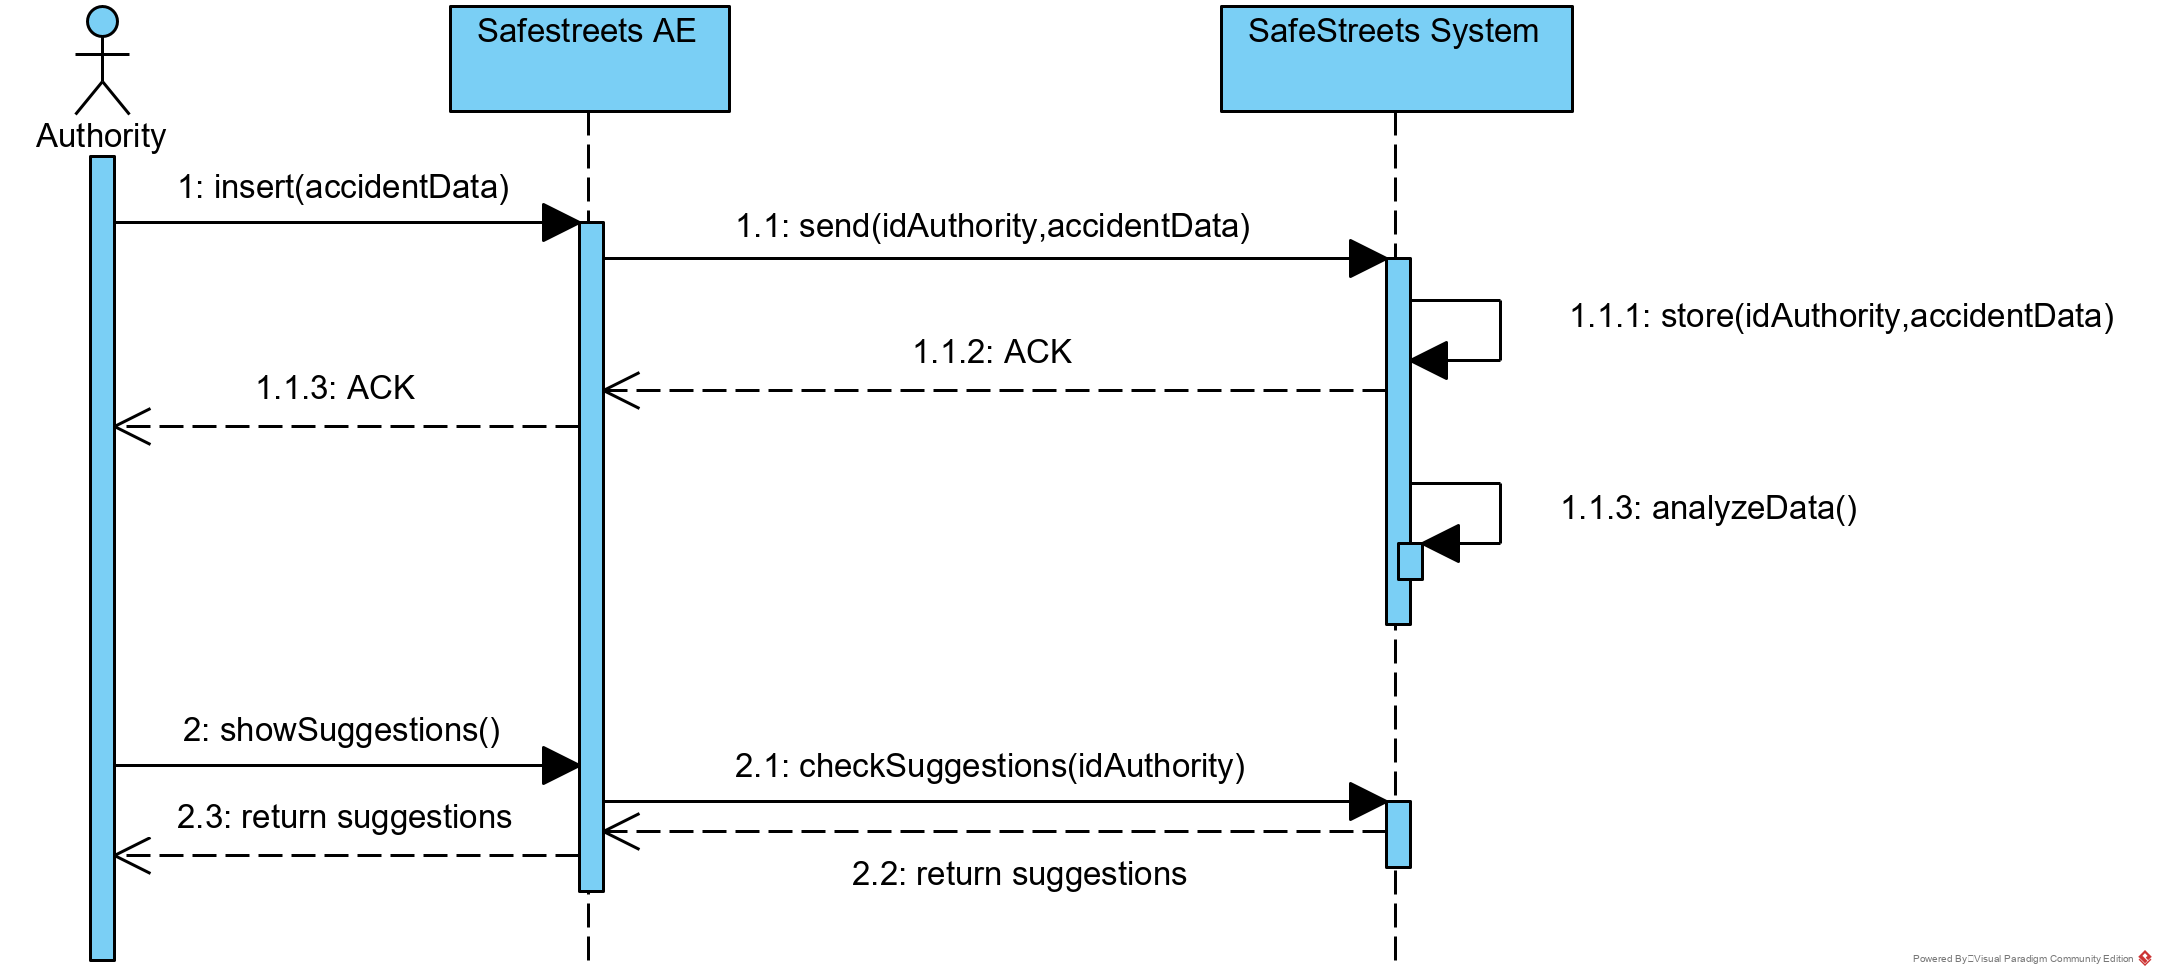
\includegraphics[width=1\textwidth]{diagrams/sequence_suggestions.png}
				\caption[SafeStreets sequence diagram]{SafeStreets sequence diagram for showing suggestions}
				\label{fig:sequencediagram_suggestions}
			\end{figure}
			
			
			
			\clearpage
			\subsubsection{Requirements traceability matrix}
				\begin{longtable}{c | c | c}
				\hline\hline
				\textbf{Goal Id} & \textbf{Use case Id} & \textbf{Requirement Id}\\
				\hline
				\multirow{3}{*}{} [G1] 
				& [UC1] & [R1] \\ \cline{3-3}
				&		& [R2] \\ \cline{3-3}
				&		& [R3] \\ \cline{3-3}
				&		& [R4] \\ \cline{3-3}
				&		& [R5] \\ \cline{3-3}
				&		& [R6] \\ \cline{3-3}
				&		& [R7] \\ \cline{3-3}
				&		& [R17] \\ \cline{3-3}
				\hline
				\multirow{3}{*}{} [G2] 
				& [UC2]	& [R8] \\ \cline{3-3}
				&		& [R9] \\ \cline{3-3}
				&		& [R10] \\ \cline{3-3}
				&		& [R11] \\ \cline{3-3}
				&		& [R12] \\ \cline{3-3}
				&		& [R13] \\ \cline{3-3}
				\hline
				\multirow{3}{*}{} [G3] 
				& [UC3] & [R14] \\ \cline{3-3}
				&		& [R15] \\ \cline{3-3}
				&		& [R16] \\ \cline{3-3}
				\hline
				\multirow{3}{*}{} [G4] 
				& [UC4] & [R18] \\ \cline{3-3}
				&		& [R19] \\ \cline{3-3}
				\hline
				\multirow{3}{*}{} [G5] 
				& [UC5] & [R20] \\ \cline{3-3}
				&		& [R21] \\ \cline{3-3}
				&		& [R22] \\ \cline{3-3}
				\hline
				\caption{Traceability matrix}
				\label{fig:Traceability matrix}
			\end{longtable}
		\clearpage
		\subsection{Performance Requirements}
			SafeStreets aims to provide a smooth user experience. For this reason, all the functionalities must be implemented so that the delay between a data request and an answer is unnoticeable, as well as the delay between the sending of a violation report and its publication.\\
			To achieve this goal, the system needs a fast internet connection. Moreover, the data sent between SafeStreets clients and servers must be compressed so to guarantee a good user experience also when the internet connection is pretty slow.\\
			In general, SafeStreets app doesn't need a lot of resources, so it can be installed on a large variety of smartphones, also dated ones.

		\subsection{Design Constraints}
		
			\subsubsection{Standards compliance}
				SafeStreets app must respect the rules of the app stores in which it will be available.\\
				Moreover, it must respect the authorization rules of the operating systems where it will be installed.\\
				
			\subsubsection{Hardware limitations}
				As mentioned in \ref{hardware_interfaces}, the application relies on some hardware components, that, if not present, doesn't allow to use SafeStreets in all its power. An external camera, a GPS service and mechanisms to connect to the internet must be present on the device to use SafeStreets.\\
				SafeStreets AE must have an internet connection of any kind and should be turned on round the clock to receive reports that have to be evaluated.
			
			\subsubsection{Any other constraint}
				SafeStreets doesn't collect personal data from its users. The only sensitive data it has to manage are the license plate associated to violation reports: they are not visible to common users, because it would make possible to associate a license plate to a particular human identity. This is not advisable: SafeStreets is an app that wants to hep authorities in finding infractions, but it doesn't want to have any impact on the reputation of people that, for any kind of reason, had done a certain number of violations.
		\subsection{Software System Attributes}
		
			\subsubsection{Reliability}
			Data collected by SafeStreets are fundamental for its functionalities. Therefore, there must be a redundant server structure to guarantee all the data about violations and accidents are never lose.
			
			\subsubsection{Availability}
			SafeStreets doesn't provide services that are critical for the life of its users. However, a user should be able to exploit SafeStreets functionalities in every part of the day, so it is interested in keeping his infrastructure active as much as possible.
			
			\subsubsection{Security}
			An information, after being stored on SafeStreets servers, is in "read-only" mode: only the state of a violation report - "confirmed" or "pending"- can be modified by external agents (precisely, by authorities). This guarantees broad security against attacks aimed at changing the meaning of the data held by SafeStreets.\\
			All communications between SafeStreets and its users use security protocols designed to guarantee the confidentiality and integrity of the communication.
			
			\subsubsection{Maintainability}
			SafeStreets source code must be well-documented and well-tested. This means that every part of the program must be commented so that its meaning is "crystal-clear", and there must be at least a 80\% coverage of the code.
			
			\subsubsection{Portability}
			SafeStreets must be implemented so that it is as much platform-independent as possible. For this reason, it won't rely on functions that are available only on particular operating systems.
	\newpage
	\section{Formal analysis using Alloy}
	
		\subsection{Purpose of the model}
		In this section some basic functionalities of SafeStreets are proved to be consistent. These are the assertions checked:
		\begin{enumerate}
			\item Every violation report received by the SafeStreets Server is complete in all its fields.
			\item Every violation report was sent to the server before the report timeout ended.
			\item When a registered authority confirms a violation report, that confirmation is consistently reported into the server.
			\item A violation report rejected by a registered authority is removed from SafeStreets database.
			\item Every accident reported by a registered authority is consistently saved into the SafeStreets database.
		\end{enumerate}
		Moreover, there are other fundamental constraints expressed so to get consistent models. For example, it is specified that every SafeStreets App is associated to one and only one user. Anyway, every constraint is straightforward or it is well commented in Alloy code.
		
		\newpage
		\subsection{Alloy model}
		\vspace{2 mm}
		\lstinputlisting[language=alloy]{alloy/worlds.als}
		\vspace{8 mm}
		
		\subsection{Checks on assertions with the Alloy Analyser}
		\begin{figure}[H]
			\centering
			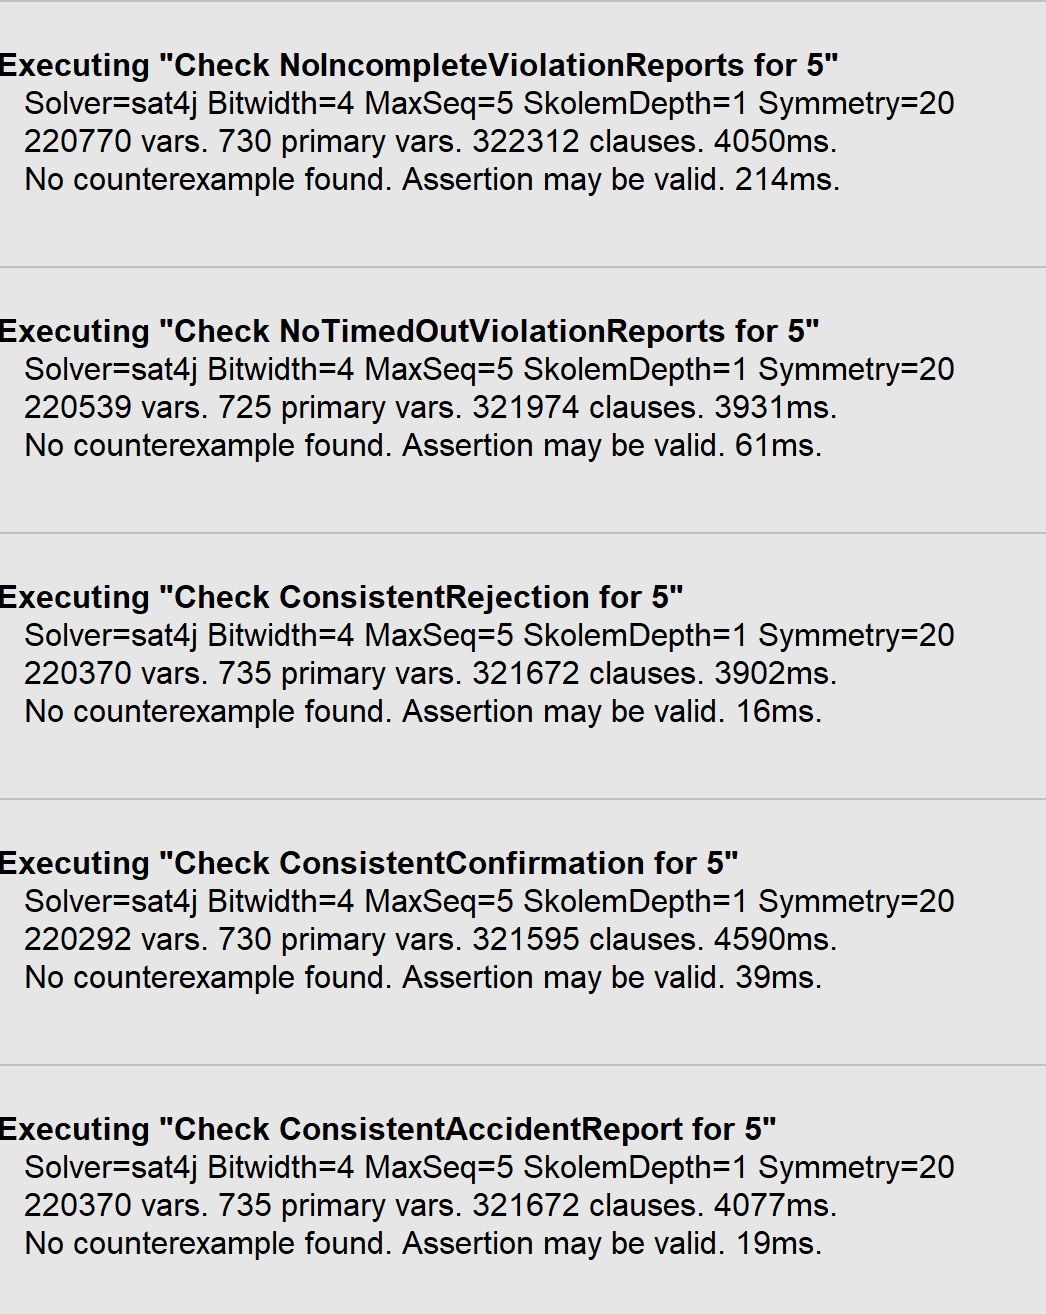
\includegraphics[width=1\textwidth]{images/AlloyAssertionsChecks.png}
			\caption[Alloy Analyser results]{These are the results of the evaluation of the assertions defined in Alloy.}
			\label{fig:check_assertions}
		\end{figure}
	
		\subsection{Worlds generated in Alloy}
		\begin{figure}[H]
			\centering
			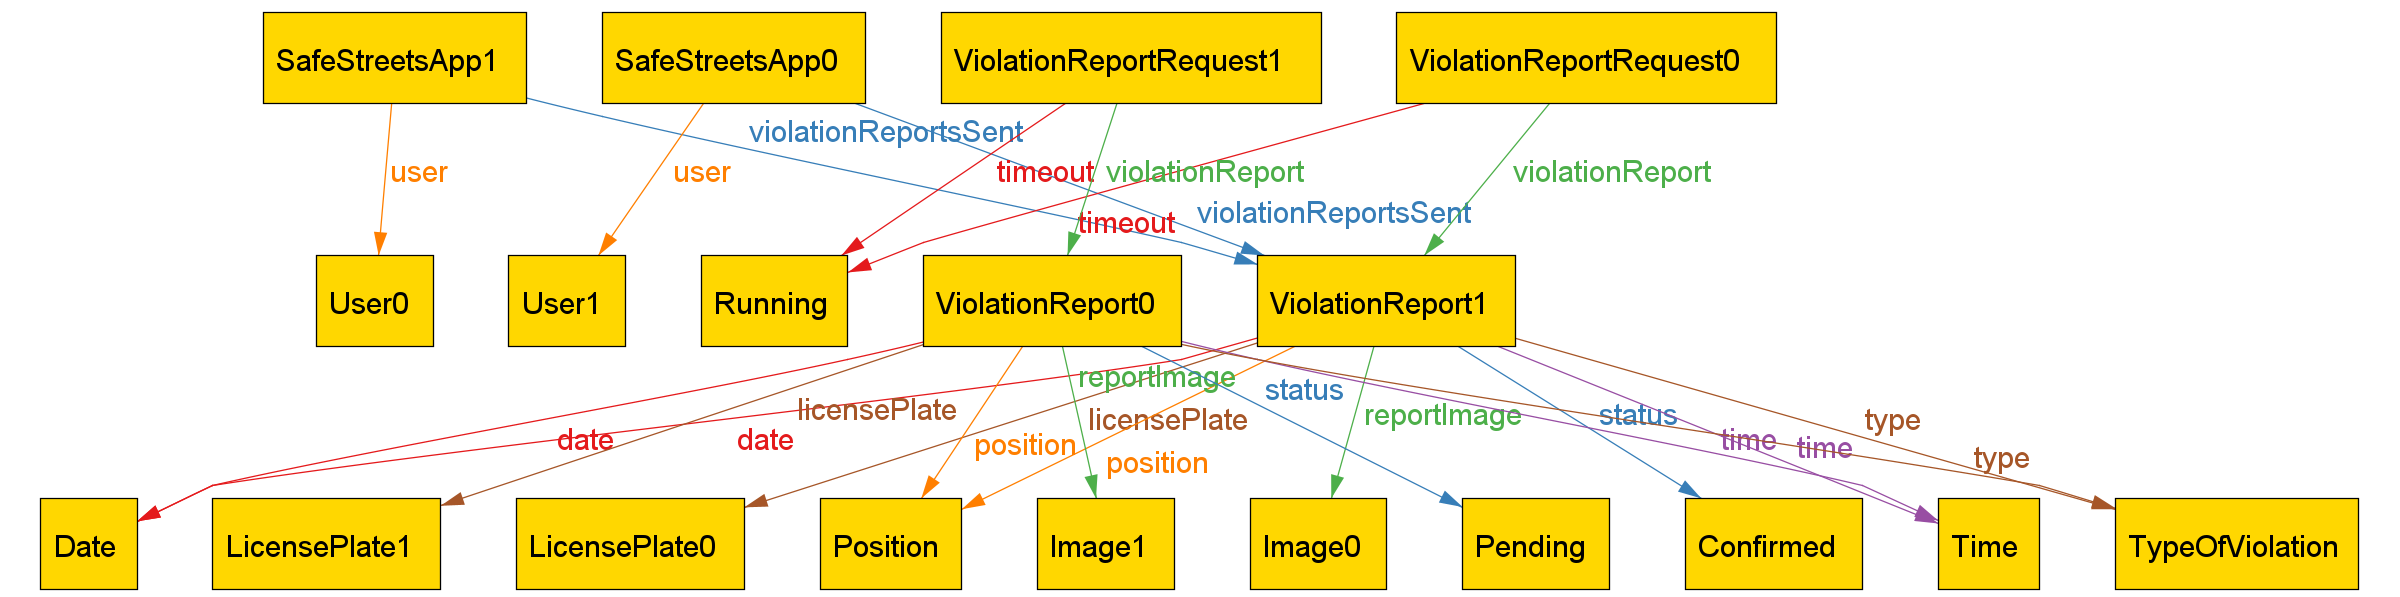
\includegraphics[width=1\textwidth]{images/alloyWorlds/world1.png}
			\caption[World 1]{This world shows the relation between the report of a violation and SafeStreets App.}
			\label{fig:alloy_world1}
		\end{figure}
		\begin{figure}[H]
			\centering
			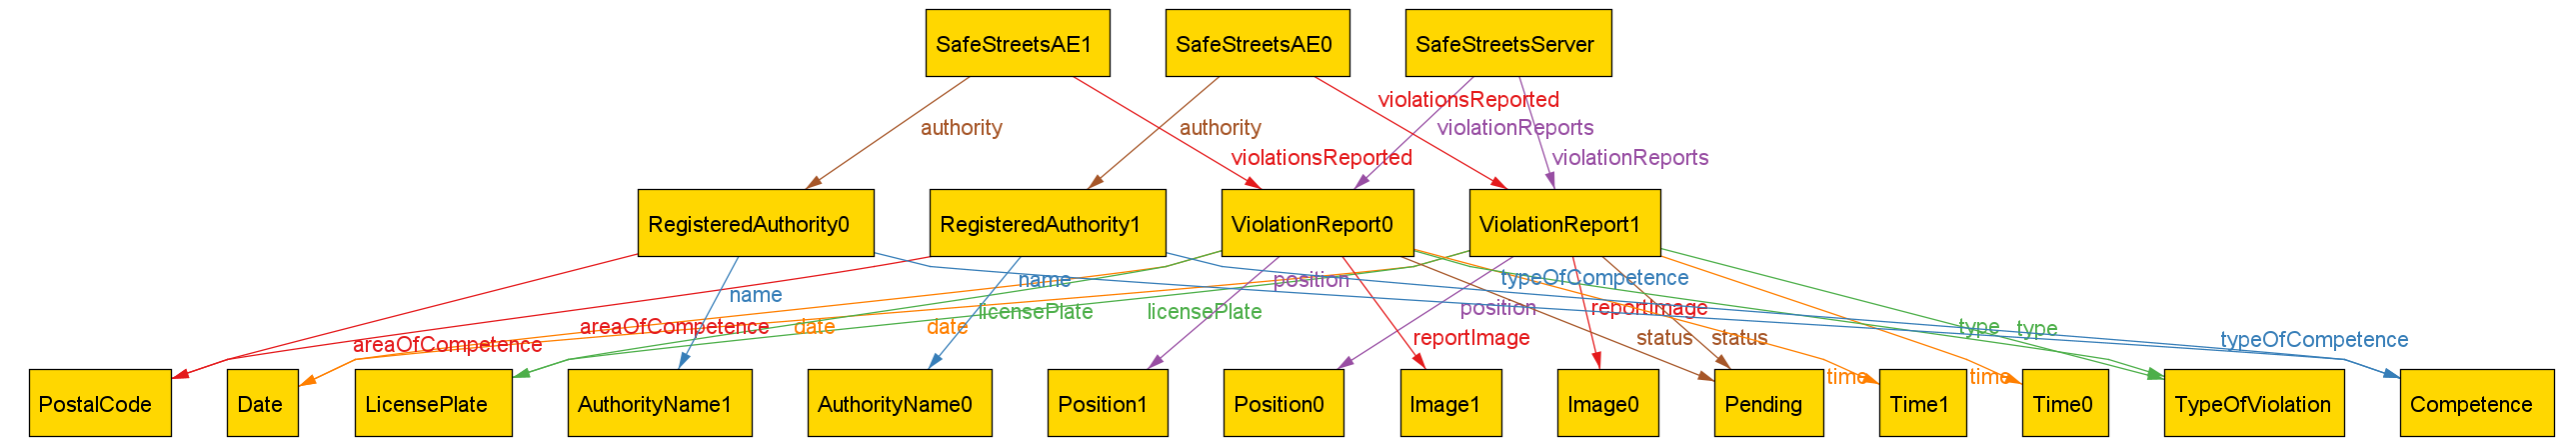
\includegraphics[width=1\textwidth]{images/alloyWorlds/world2.png}
			\caption[World 2]{This world shows the relation between the SafeStreets server and SafeStreets AE's in violation report evaluation.}
			\label{fig:alloy_world2}
		\end{figure}
		\begin{figure}[H]
			\centering
			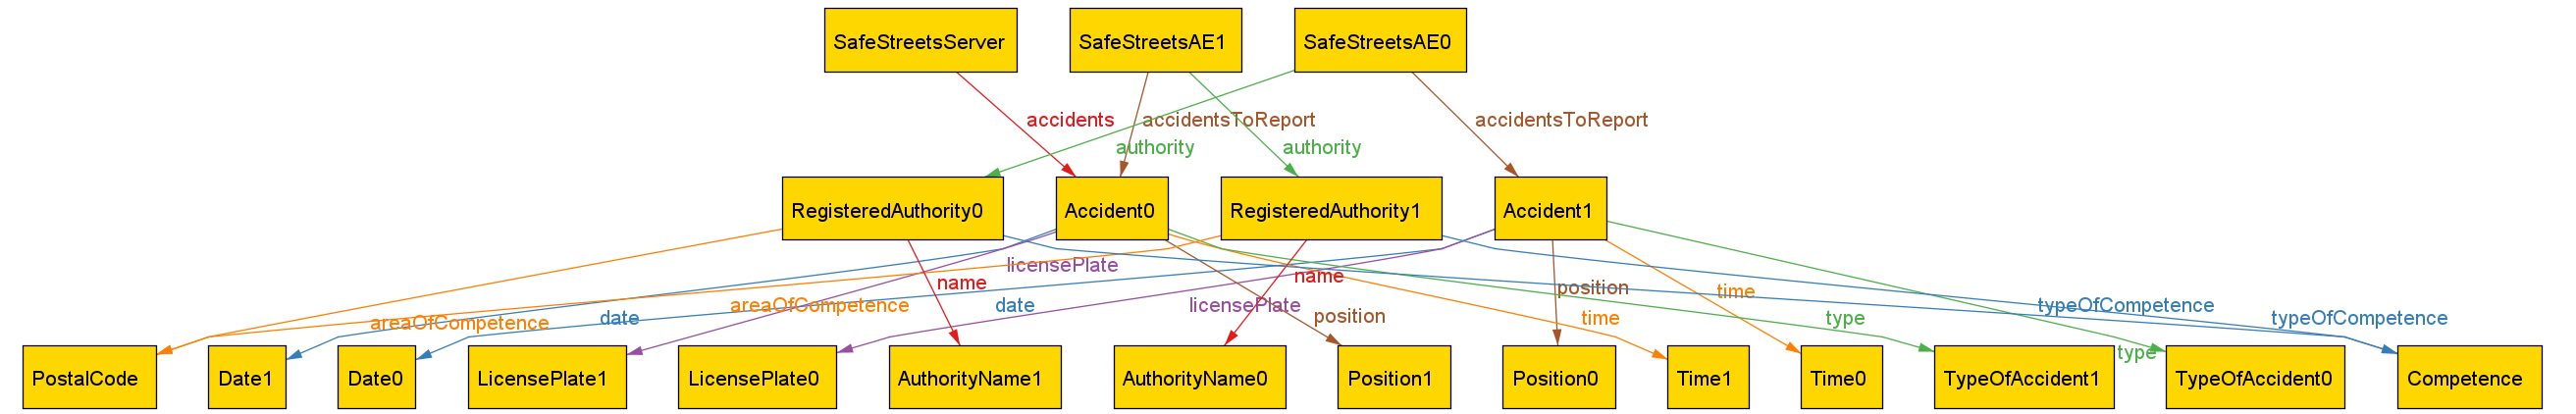
\includegraphics[width=1\textwidth]{images/alloyWorlds/world3.png}
			\caption[World 3]{This world shows the relation between the SafeStreets server and SafeStreets AE's in reporting accidents.}
			\label{fig:alloy_world3}
		\end{figure}
		
		\newpage
	\section{Effort spent}
	\begin{table}[h]
		\centering
		\begin{tabular}{l c}
			\hline\hline
			\multicolumn{2}{c}{\textbf{Team Work}} \\
			\hline
			\textbf{Task} & \textbf{Hours} \\ [0.5ex]
			\hline
			Understanding the problem & 2  \\
			Brainstorming & 4 \\
			Software system attributes & 8 \\
			\hline
			\textbf{Total} & 14  \\
			\hline
		\end{tabular}
		\caption{Time spent by all team members}
		\label{fig:Time spent by all team members}
	\end{table}
	
	\begin{table}[h]
		\centering
		\begin{adjustbox}{width=1\textwidth}
			\begin{tabular}{l c l c l c}
				\hline\hline
				\multicolumn{6}{c}{\textbf{Individual Work}} \\
				\hline
				\multicolumn{2}{c |}{\textbf{Nicolò Sala}}  &
				\multicolumn{2}{c |}{\textbf{Sebastiano Quacquarelli}} &
				\multicolumn{2}{c}{\textbf{Simone Ricchiuti}}\\
				\hline
				\textbf{Task} & \textbf{Hours}
				& \textbf{Task} & \textbf{Hours}
				& \textbf{Task} & \textbf{Hours} \\ [0.5ex]
				\hline
				%Nicolò								Sebastiano							Simone
				Constraints & 2						& Definitions & 1					& Introduction & 4
				\\\hline
				Definitions & 1						& User interfaces. & 5				& Product functions  & 4
				\\\hline
				UC description & 3					& Domain model & 4				    & User characteristics  & 0.5 
				\\\hline
				Performance req. & 1				& UC descr./diagrams & 4			& Functional req & 2 
				\\\hline
				Design constraints & 1				& Assumptions & 2					& UC description & 3  
				\\\hline
				Alloy & 9							& Sequence diagrams & 3				& Activity Diagrams  & 2  
				\\\hline
				\textbf{Total} & 17					& \textbf{Total} & 19				& \textbf{Total} & 15.5
				\\\hline
			\end{tabular}
		\end{adjustbox}
		\caption{Time spent by each team member}
		\label{fig:Time spent by each team member}
	\end{table}
	
	\newpage
	\section{References}
	\begin{itemize}
		\item "2019-2020 Software Engineering 2 mandatory project: goal, schedules and rules";
		\item TeXstudio (\url{https://www.texstudio.org}) to edit the LaTeX document;
		\item Overleaf (\url{https://www.overleaf.com}) also to edit the LaTeX document;
		\item AlloyTools (\url{https://www.alloytools.org}) to learn how to use Alloy and to download Alloy 5;
		\item Visual Paradigm CE (\url{https://www.visual-paradigm.com/}) to create UML diagrams.
		\item Mockplus Free (\url{https://www.mockplus.com/}) to design prototypes of user interface.
	\end{itemize} 
\end{document}
